% https://www.overleaf.com/13649083bgsrpnmkdxgp#/52781645/

\documentclass[compress]{beamer}
\usetheme{Warsaw}


\setbeamertemplate{headline}{%
\leavevmode%
  \hbox{%
    \begin{beamercolorbox}[wd=0.92\paperwidth,ht=2.5ex,dp=1.5ex]{palette quaternary}%
    \insertsectionnavigationhorizontal{\paperwidth}{}{\hskip0pt plus1filll}
    \end{beamercolorbox}%
    \begin{beamercolorbox}[wd=.08\paperwidth,ht=2.5ex,dp=1.5ex,leftskip=.3cm,rightskip=.3cm plus1fil]{title in head/foot}%
    \usebeamerfont{title in head/foot}\hfill\insertframenumber\,/\,\inserttotalframenumber
  \end{beamercolorbox}}
          %}
}
\setbeamertemplate{footline}{}
%OR

%\defbeamertemplate*{footline}{shadow theme}
%{% this section is for frame numbering
  %\leavevmode%
  %\hbox{\begin{beamercolorbox}[wd=.5\paperwidth,ht=2.5ex,dp=1.125ex,leftskip=0.3cm plus1fil,rightskip=0.3cm]{author in head/foot}%
   % \usebeamerfont{author in head/foot}
  %\end{beamercolorbox}%
  %\begin{beamercolorbox}[wd=.5\paperwidth,ht=2.5ex,dp=1.125ex,leftskip=.3cm,rightskip=.3cm plus1fil]{title in head/foot}%
   % \usebeamerfont{title in head/foot}\hfill\insertframenumber\,/\,\inserttotalframenumber
  %\end{beamercolorbox}}%
 %\vskip0pt%
%}


\usecolortheme{spruce}
\usepackage[french]{babel}
\usepackage[utf8]{inputenc}
\usepackage[T1]{fontenc}
\usepackage{lmodern}
\usepackage{tikz} % pour rendre figures transparentes
\usetikzlibrary{positioning,backgrounds}   % here to test diagram
\usepackage{graphicx}
\usepackage{enumerate}  % to enumerate
% \usepackage{amsmath,empheq}% to use crochet mathématiques and symbole degree
\usepackage[absolute,overlay]{textpos}% pour la fonction textblock
\setbeamertemplate{frame numbering}[fraction]
\usepackage{listings}
\usepackage{color}
\definecolor{green1}{rgb}{0.13, 0.55, 0.13}
\definecolor{gray}{rgb}{0.92,0.92,0.92}

\setbeamertemplate{itemize item}{\color{green1}$\bullet$}  %change color+forme item
\setbeamertemplate{itemize subitem}{\color{green1}$\circ$}
\setbeamertemplate{itemize subsubitem}{\color{green1}$\diamond$}
  
  \usepackage{listings}   %to use listings - use [fragile] on frame 
 \usepackage{ragged2e} % !! césure mots
 \apptocmd{\frame}{}{\justifying}{} %allow justifying
   

%for R code inside presentation
\lstset{frame=tb,
  backgroundcolor=\color{gray},
  language=R,
  aboveskip=3mm,
  belowskip=3mm,
  showstringspaces=false,
  columns=flexible,
  basicstyle={\small\ttfamily},
  numbers=none,
  breaklines=true,
  breakatwhitespace=true,
  tabsize=3
}
\begin{document}
\newcommand{\un}{\textunderscore}
%%%%%%%%%%%%%%%%%%%%%%%%%%%%%%%%%%%%%%%%%%%%%%%%%
%%%%%%%%%%%%%%%%%%%%%%%%%%%%%%%%%%%%%%%%%%%%%%%%% (Title)
\setbeamertemplate{navigation symbols}{}  %delete navigation symbol

\title[The evolutionary dynamics of laying date]{The evolutionary dynamics of laying date \\ in the pied flycatcher \textit{Ficedula hypoleuca}} 
\subtitle{PhD defense}
\author{\textbf{Justine Le Vaillant}}
\date{ \small 17$^{th}$December 2021}
\institute{PhD Supervisor : Jes\'{u}s Mart\'{i}nez-Padilla \\
  Academic tutor : Pedro Abellán}
%\begin{textblock*}{10cm}(0.5cm,8.5cm)
%\vspace{0.3pt}
 %\includegraphics[width=0.95\paperwidth]{Image/friselab.png}
%\end{textblock*}


%%%%%%%%%%%%%%%%%%%%%%%%%%%%%%%%%%%%%%%%%%%%%%%%
\usebackgroundtemplate{%
%\tikz\node[opacity=0.35] %{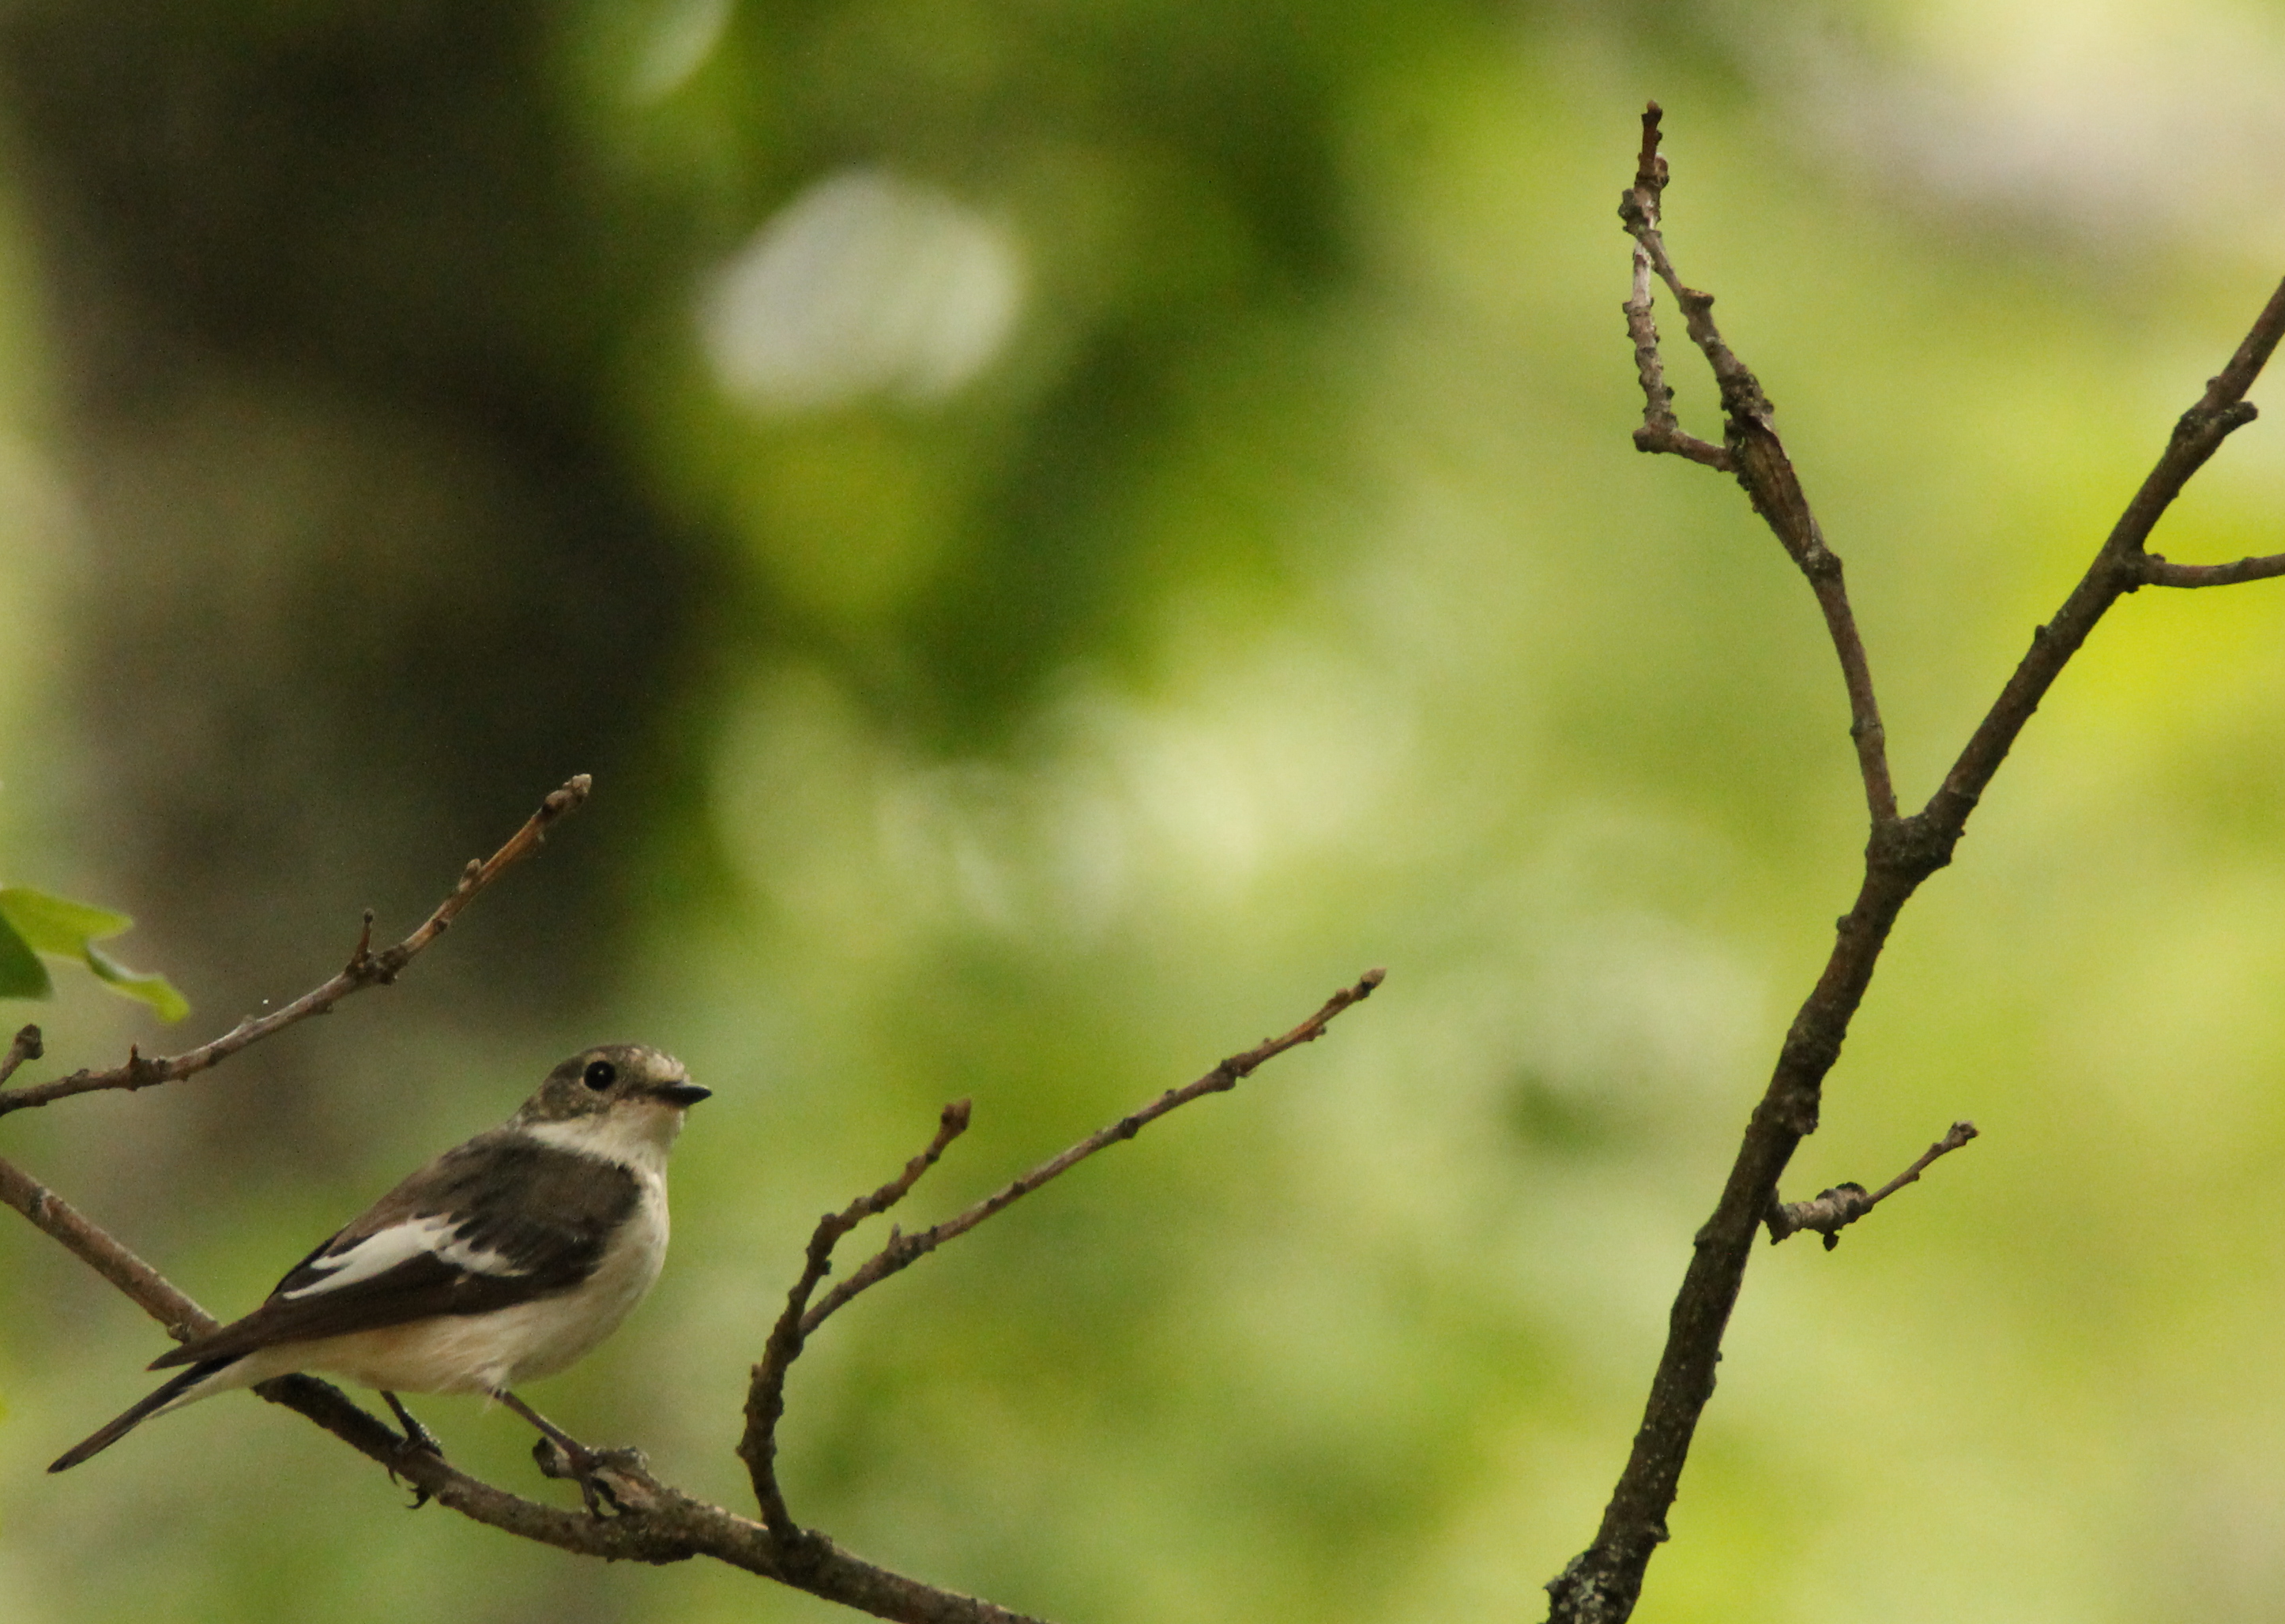
\includegraphics[height={\paperheight},width=\paperwidth]{Photos/back2.png}};}
{\includegraphics[height={\paperheight},width=\paperwidth]{Image/Illustration/Background.png}};}

{
\setbeamertemplate{footline}{}  %to avoid footline on the title page
\setbeamertemplate{headline}{} 

\begin{frame}
  \titlepage
\end{frame}
}
\addtocounter{framenumber}{-1}
\usebackgroundtemplate{} % from here, white fond blanc

%%%%%%%%%%%%%%%%%%%%%%%%%%%%%%%%%%%%%%%%%%%%%%%%
%%%%%%%%%%%%%%%%%%%%%%%%%%%%%%%%%%%%%%%%%%%%%%%%%
\section{Introduction}
\begin{frame}{General Introduction}\vspace{10pt}

\raggedright
\textbf{Evolution:} change in the frequency distribution of alleles or heritable phenotypes. \\
 \vspace{0.3cm}
 \centering

 \begin{tikzpicture}
    \begin{scope}[blend group = soft light]
    \fill[red!30!white]   ( 90:1.2) circle (2);
    \fill[green!30!white] (210:1.2) circle (2);
    \fill[blue!30!white]  (330:1.2) circle (2);
  \end{scope}
  \node at ( 90:2)    {Selection};
  \node at ( 210:2)   {Variability};
  \node at ( 330:2)   {Heritability};
  \node [font=\Large] {Evolution};
  \end{tikzpicture}
  
\end{frame}
%%%%%%%%%%%%%%%%%%%%%%%%%%%%%%%%%%%%%%%%%%%%%
\begin{frame}{General Introduction}

\textbf{Phenotypic selection} is shaped by the relation between relative fitness and phenotypic variation in a population.\\
 \vspace{0.2cm}
 \centering
 \includegraphics[height = 5.5 cm]{Image/Phenotypic change.jpg} \\
 \raggedleft \tiny{Lande \& Arnold 1983, \textit{Evolution}} \\
  
\vspace{0.1cm}
\raggedright\normalsize
Natural selection can impact genetic variation on a trait \centering$\Longrightarrow$\textbf{Evolution}.

\end{frame}

%%%%%%%%%%%%%%%%%%%%%%%%%%%%%%%%%%%%%%%%%%%%%%%%%
\begin{frame}{General Introduction}

%\textbf{Natural selection:} process that causes population to change over time,  a mechanism that induce a change in the frequency distribution of alleles that favours local adaptation. \\
%The ecological causes of evolution can be 
 
The direction or strength of \textbf{natural selection} can be affected by changes in abiotic and biotic \textbf{environmental conditions}, and  have an evolutionary impact on populations.

\vspace{0.5cm}\centering
 \includegraphics[height = 6 cm]{Image/Illustration/env condition.png} \\




\end{frame}
%%%%%%%%%%%%%%%%%%%%%%%%%%%%%%%%%%%%%%%%%%%%%%%%%%%%%
\begin{frame}{General Introduction}\vspace{10pt}

Evolution occurs in an ecological context (\small\textit{eco-evolutionary dynamic}).\\
 \vspace{0.5cm}
 \normalsize
Evolutionary change can be induced by adaptive forces like natural selection but it is caused by \textbf{environmental variation}. \\

 \vspace{0.5cm}
 \centering
 \includegraphics[height = 3.2 cm]{Image/1976.jpg}
 \includegraphics[height = 3.2 cm]{Image/1978.jpg}\\
 \raggedleft
\vspace{0.1cm}
\tiny
 %Grant & Grant (1995). Predicting microevolutionary responses to directional selection on heritable variation. \textit{Evolution}, 49(2), 241–251.
Grant \& Grant 1995, \textit{Evolution}

\vspace{0.3cm}
\raggedright\normalsize
Evolution by natural selection is a continuous and gradual process that usually leads to  \textbf{local adaptation}.

\end{frame}


%%%%%%%%%%%%%%%%%%%%%%%%%%%%%%%%%%%%%%%%%%%%%%%%%
\begin{frame}{General Introduction}\vspace{10pt}

In a context of Climate Change, the challenge is predicting and detecting local adaptation.\\
\vspace{0.3cm}
\onslide<2->{
 \textbf{Microevolution:} evolutionary (genetic) change in a population over relatively short periods of time. \\ 
 \centering
 %\includegraphics[height = 1.5 cm]{Image/Illustration/microevol.png}
 %\includegraphi
 \includegraphics[height = 2 cm]{Image/Illustration/microevolution.png}
  }\\ \onslide<3->{\\
 %\vspace{0.1cm}
  \raggedright
  %lack of genetic change =! lack of adaptation = PP
 \textbf{Phenotypic plasticity:} Variation in the expression of phenotypes by the same genotype in a gradient of environmental conditions.\\
 \centering
 \includegraphics[height = 2.3 cm]{Image/Plasticity1.png}
 }
\end{frame}

%%%%%%%%%%%%%%%%%%%%%%%%%%%%%%%%%%%%%%%%%%%%%%%
\begin{frame}{General Introduction}\vspace{10pt}

\begin{itemize}
\item How and how fast, natural populations may respond to
environmental changes? 
\item What is the evolutionary impact of environmental change on wild animal populations?
\item Can local adaptation buffer the influence of climate change?
\item May plasticity favour local adaptation?
\end{itemize}

 \vspace{0.5cm}
 \centering
 \onslide<2->{
 \begin{tabular}{ccc}
   \includegraphics[height = 2 cm]{Photos/Red-billed_gull,_Red_Zone,_Christchurch,_New_Zealand.jpg} &
 \includegraphics[height = 2 cm]{Photos/Tamiasciurus hudsonicus.jpg}&
 \includegraphics[height = 2 cm]{Photos/320px-European_Common_Frog_Rana_temporaria_(cropped).jpg}
    \\[\abovecaptionskip]
  Body size & Partuition date & Growth rate
    \\\tiny{
Teplisky \textit{et al.} 2008, \textit{PNAS}\hspace{0.5cm}}&
     \tiny{Réale \textit{et al.} 2003,  \textit{Evolution}\hspace{0.5cm}} &
     \tiny{Orizaola \textit{et al.} 2010, \textit{Ecography}}
\end{tabular}
}

%see in Merilä \& Hendry 2014 \textit{Evolutionary Applications}
\end{frame}

%%%%%%%%%%%%%%%%%%%%%%%%%%%%%%%%%%%%%%%%%%%%%%%%%
\begin{frame}{General Introduction}\vspace{10pt}

\textbf{Laying Date:} Day of the first laid egg: it determines breeding time and reproductive success (\textit{fitness}). \\
 \vspace{0.5cm}
 \centering
 \includegraphics[height = 4 cm]{Image/timing breeding.png}

\end{frame}


%%%%%%%%%%%%%%%%%%%%%%%%%%%%%%%%%%%%%%%%%%%%%%%%%

\begin{frame}{General Introduction}\vspace{10pt}

\raggedright
\textbf{Phenology:} Periodic life-cycle events that are influenced by seasonal and inter-annual variations in climate.\\
\vspace{0.5cm}
Increasing temperatures may force birds to start laying earlier. \\
 \vspace{0.3cm}
 \centering
  \only<1>{\includegraphics[height = 4.5 cm]{Image/Phenology change.png}}
 \only<2>{ \includegraphics[height = 4.5 cm]{Image/Phenology change2.png}}
 \\

\raggedleft
\vspace{0.1cm}
\tiny
Both \textit{et al.} 2004, \textit{Proc. R. Soc. Lond., B, Biol. Sci.}\\
Visser \textit{et al.} 2006, \textit{Oecologia} 
  
\end{frame}

%%%%%%%%%%%%%%%%%%%%%%%%%%%%%%%%%%%%%%%%%%%%%%%%
\begin{frame}{General Introduction}\vspace{10pt}

\begin{textblock*}{6cm}(0.3cm,1.5cm)

Migrant species are more constrained to advance laying date under events of climate change.
\vspace{0.2cm}

%\centering
\includegraphics[height = 4 cm]{Image/migrant2.png} \\
 \scriptsize \textbf{1} Resident \textbf{2} short-distance migrant and \\ \textbf{3} long-distance migrant species\\
\raggedleft
\vspace{0.1cm}
  % \tiny{Kluen, E., Nousiainen, R., \& Lehikoinen, A. (2017). Breeding phenological response to spring weather conditions in common Finnish birds: resident species respond stronger than migratory species. Journal of Avian Biology, 48, 611–619.} \\
  \tiny{Kluen \textit{et al.} 2017, \textit{Journal of Avian Biology}} \\

\end{textblock*}

  \only<2->{
\begin{textblock*}{5cm}(7cm,2cm)

Within-species and populations differences in plasticity and \\ response to climate change.\\
\vspace{0.6cm}
 \centering
 \includegraphics[height = 2.5 cm]{Image/difference.png} \\
 \scriptsize \textbf{A} UK and \textbf{B} Dutch \\ great tits population \\
 \raggedleft
\vspace{0.1cm}
  % \tiny{Charmantier A., McCleery R.H., Cole L.R., Perrins C., Kruuk L.E., Sheldon B.C. (2008) Adaptive phenotypic plasticity in response to climate change in a wild bird population. Science 320: 800–803.} \\
  \tiny{Charmantier \textit{et al.} 2008, \textit{Science}} \\

\end{textblock*}
}
\end{frame}

%%%%%%%%%%%%%%%%%%%%%%%%%%%%%%%%%%%%%%%%%%%%%%%%
%%%%%%%%%%%%%%%%%%%%%%%%%%%%%%%%%%%%%%%%%%%%%%%%
%%%%%%%%%%%%%%%%%%%%%%%%%%%%%%%%%%%%%%%%%%%%%%%%%
\begin{frame}{Objectives}
   \begin{enumerate}
   \setbeamercolor{item projected}{bg=green!30!white,fg=black}
  \setbeamertemplate{enumerate items}[circle]
   \small
\item Is the expression of a labile trait predictable among individuals and time? \\
\onslide<2->{\textbf{Chapter I} %: Repeatability of reproductive events
  }
\vspace{0.3cm}

\setbeamercolor{item projected}{bg=red!30!white,fg=black}
  \setbeamertemplate{enumerate items}[circle] 
\item What are the environmental factors that shape selection on laying date? \\
\onslide<2->{\textbf{Chapter II} }%: Detecting the relative influence of environmental variables in selection on laying date  
\vspace{0.3cm}

\setbeamercolor{item projected}{bg=blue!30!red!30!white,fg=black}
  \setbeamertemplate{enumerate items}[circle]
\item Can environmental variation shape genetic changes of laying date in short-time periods? \\
\onslide<2->{\textbf{Chapter III}} %: Response to selection and evolutionary change
\vspace{0.3cm}

\setbeamercolor{item projected}{bg=blue!30!white,fg=black}
  \setbeamertemplate{enumerate items}[circle]
\item  Can phenotypic plasticity evolve under different environmental factors? \\
\onslide<2->{\textbf{Chapter IV}} %: Genetic merit of plasticity on local adaptation
\vspace{0.3cm}

\setbeamercolor{item projected}{bg=green!30!white,fg=black}
  \setbeamertemplate{enumerate items}[circle]
\item  To what extent within-individual variation may explain total variance of laying date under changing environmental conditions? \\
\onslide<2->{\textbf{Chapter V}}% : Phenotypic, genetic and individual variation
\end{enumerate}
  \end{frame}


%%%%%%%%%%%%%%%%%%%%%%%%%%%%%%%%%%%%%%%%%%%%%%%
\section{Material}
\begin{frame}{Population study}

\begin{textblock*}{9cm}(2.5cm,1cm)
\begin{figure}
 \small Pied flycatcher, \textit{Ficedula hypoleuca}
\includegraphics[width = 5 cm]{flycatcher2.png} 
\end{figure}
\end{textblock*}

\vspace{2.5cm}
Small passerine bird, insectivorous, migrant

\begin{center}
 \includegraphics[height = 3.5 cm]{Image/Illustration/map1.png} 
    \end{center}

Long-term study: population monitored between 1987 and 2016 in Central Spain \textit{La Hiruela} (2 forests areas, 237 nest-boxes)

\end{frame}
%%%%%%%%%%%%%%%%%%%%%%%%%%%%%%%%%%%%%%%%%%%%%%%%%

\begin{frame}{Population study}

\begin{figure}
\centering
      \includegraphics[height = 7 cm]{Image/map.png} 
\end{figure}
\raggedleft
      % \tiny{Both, C. \& te Marvelde L. (2007). Climate change and timing of avian breeding and migration throughout Europe. Climate Research, 35(1–2), 93–105.}
      \tiny{Both \& te Marvelde 2007, \textit{Climate Research}}

\end{frame}
%%%%%%%%%%%%%%%%%%%%%%%%%%%%%%%%%%%%%%%%%%%%%%%
\begin{frame}{Population study}\vspace{10pt}

\begin{textblock*}{10cm}(1cm,1.3cm)
29 years of a monitored population (3021 obs; 1599 Females):
%  
\end{textblock*}

\begin{textblock*}{9cm}(0.5cm,1.7cm)
\begin{itemize}
\item<2->Life-history traits
\begin{itemize}
\item Phenology (laying date)
\item Fitness (recruits)
\end{itemize}

\item<3-> Morphological traits 
\begin{itemize}
\item Body size (tarsus length [0.01mm])
\item Body mass [g] 
\end{itemize}

\item <4->Individuals data 
\begin{itemize}
\item Age (one year old or older)
%\item Mate (male identity)
\item Polygamous status
\item Level of relatedness (social pedigree)
\end{itemize}
\end{itemize}
\end{textblock*}

\begin{textblock*}{6cm}(6cm,2cm)
\onslide<2->{\raggedleft\includegraphics[height = 4.1cm]{Image/cycle.jpg}}
\end{textblock*}

\vspace{5cm}
\centering
 \onslide<3->{ \includegraphics[height = 2.25cm]{Photos/tarsus.jpg}}
 \onslide<4->{\includegraphics[height = 2.25cm]{Photos/age.jpg}}
  \onslide<4->{\includegraphics[height = 2.25cm]{Photos/blood.jpg}}
\end{frame}

%%%%%%%%%%%%%%%%%%%%%%%%%%%%%%%%%%%%%%%%%%%%%%%%%

\begin{frame}{Population study}

\centering
  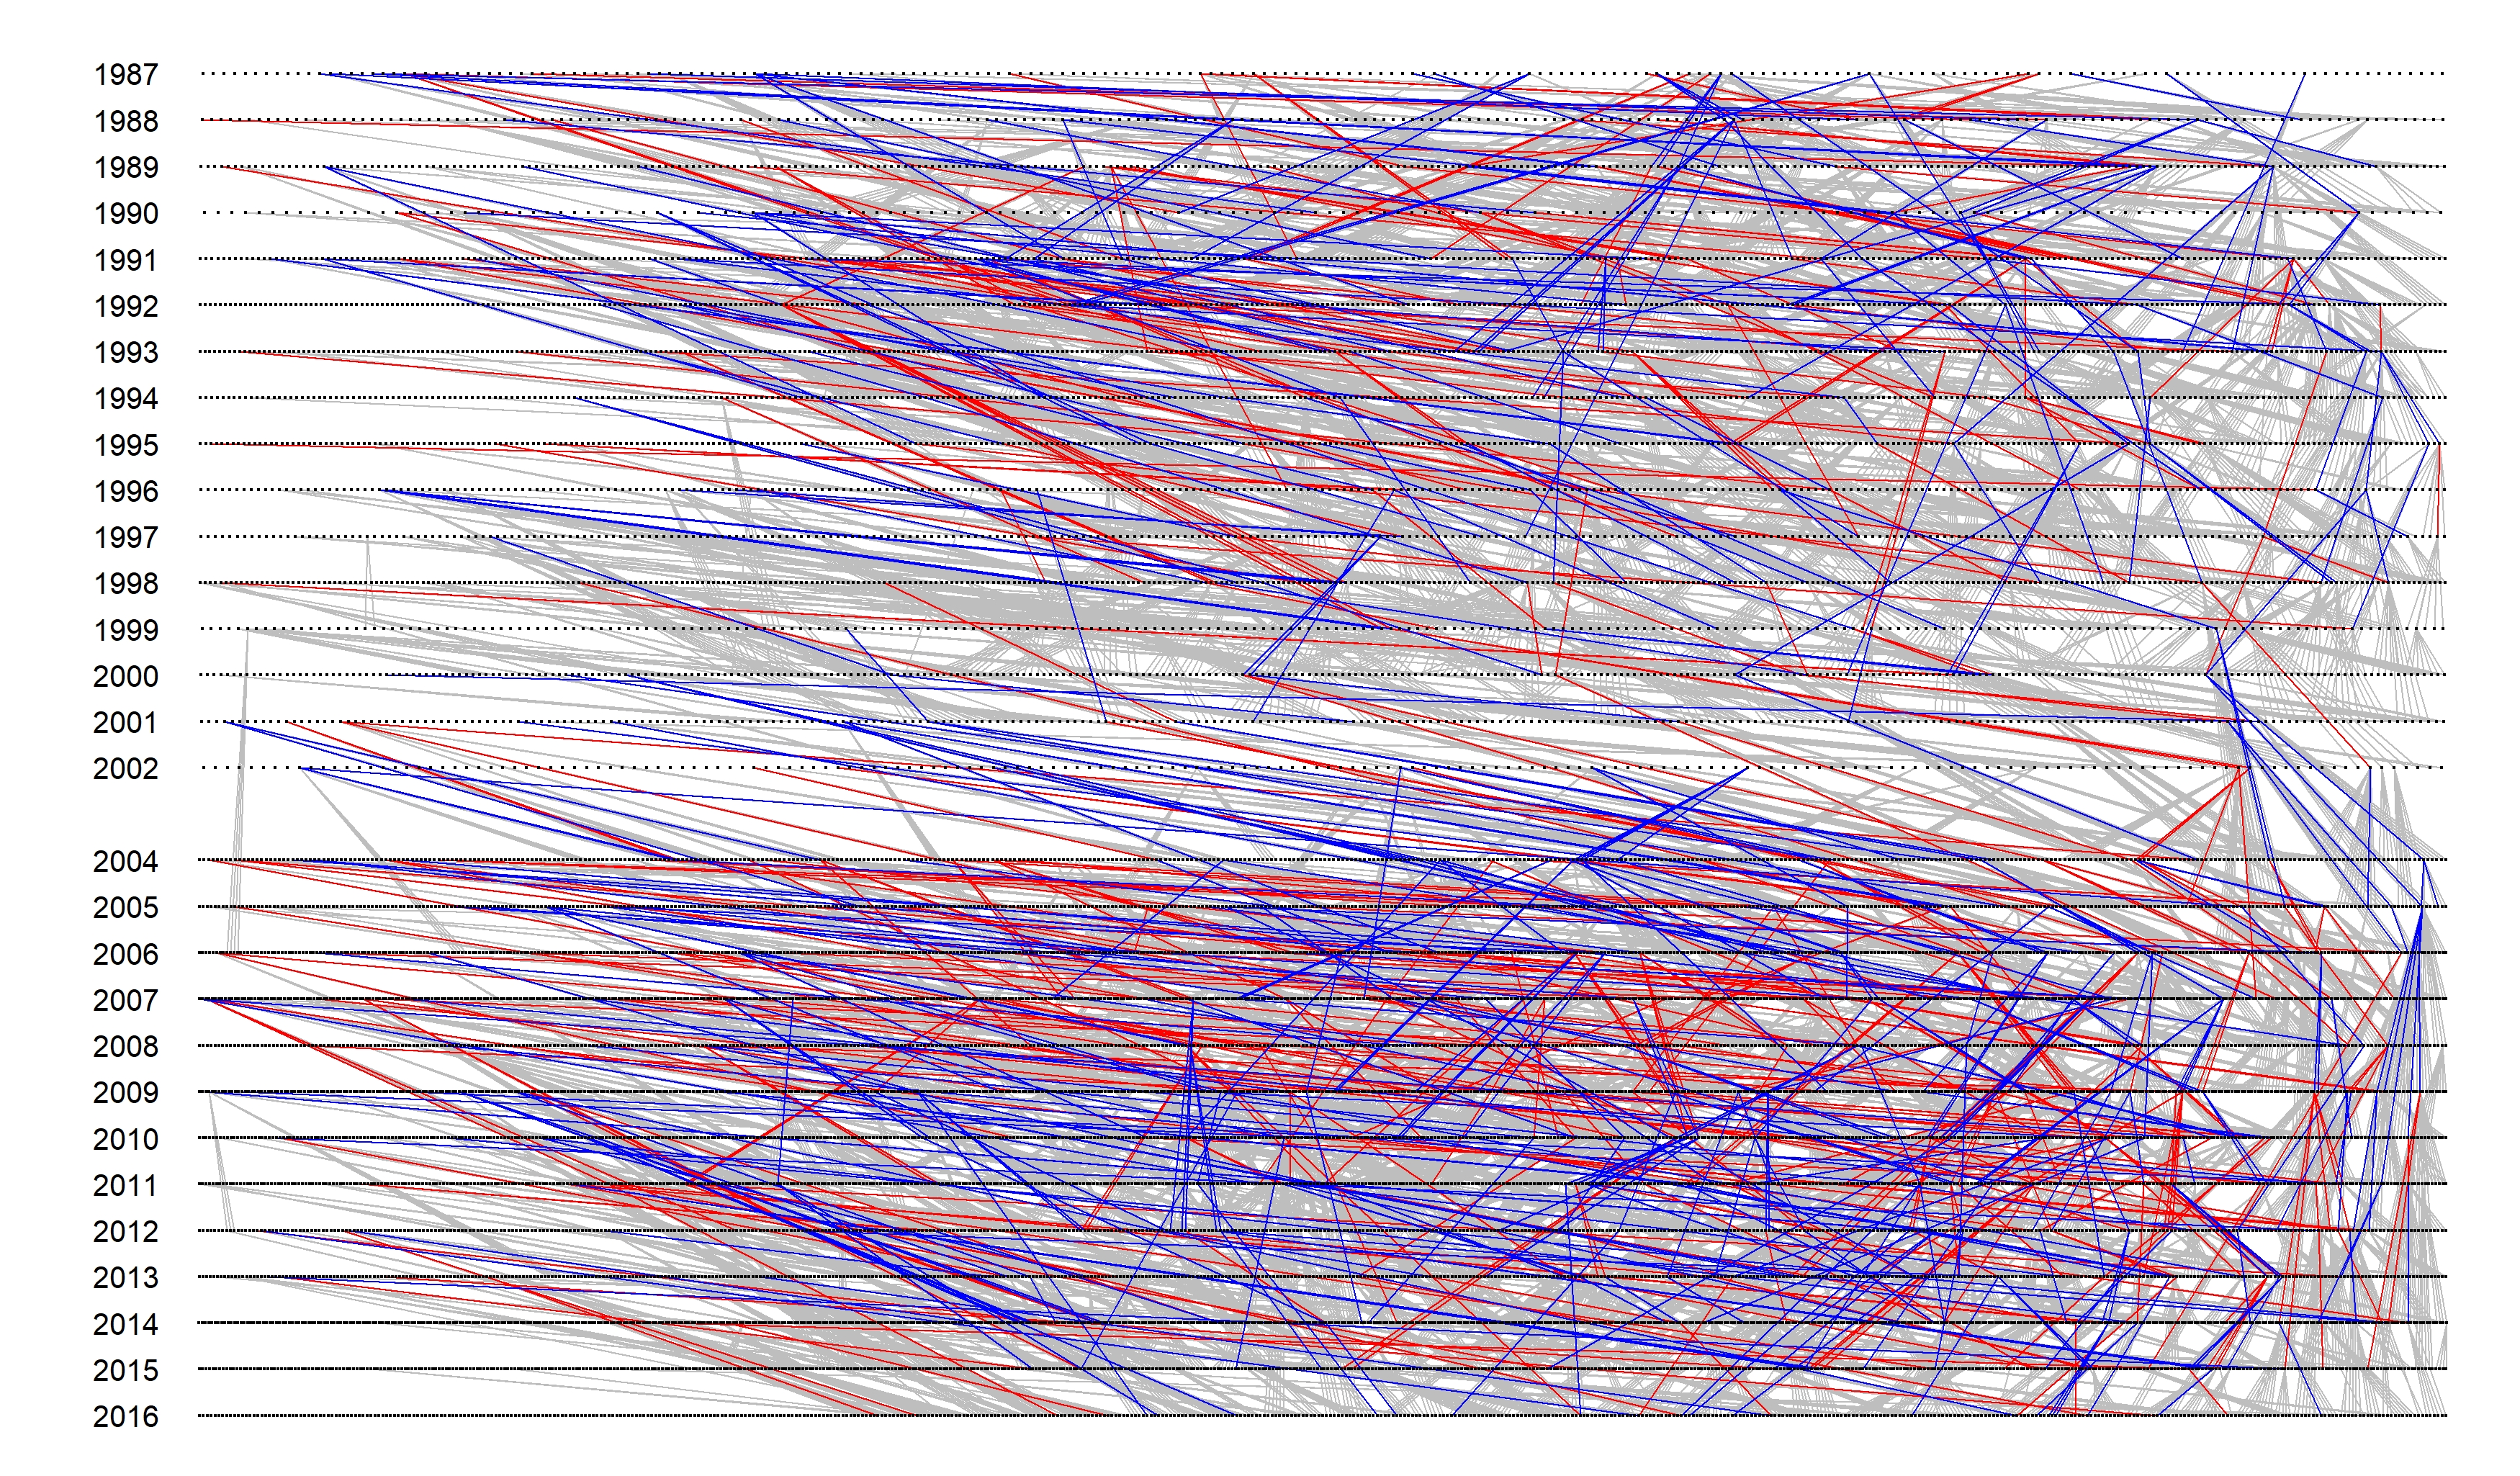
\includegraphics[height = 6.5cm]{Image/Cohort.jpg} \\
\vspace{0.1cm}
\small Individual degree of relatedness (\textbf{social pedigree}):\\
13 generations with 1 599 maternities (red), 1 454 paternities (blue),\\ 13 266 offsprings (grey) for 1 089 females recruits (color)


\end{frame}


%%%%%%%%%%%%%%%%%%%%%%%%%%%%%%%%%%%%%%%%%%%%%%%%%%%%%%%%%%%%%%%%%%%%%%%%%%%%%%%%%%%%%%%%%%%%%%%%%
\section{Methods}
\begin{frame}{Methods}

\raggedright
\textbf{"Animal model":} Mixed model that teases apart the \textbf{total phenotypic variance $V_P$} into \textbf{additive genetic variance $V_A$} and other sources of variance (environmental, year, individual, etc) by including a matrix of relatedness (\textbf{pedigree}) \texttt{as random factor}.\\

\vspace{0.2cm}
 \begin{exampleblock}{Quantitative genetic models}
\[ V_P=V_G + V_E\] 

\scriptsize 
$V_P$: Total phenotypic variance\\
$V_G$: Genetic variance = \textbf{$V_A$: Additive genetic variance} + non-additive variance\\
$V_E$: Non-genetic variance : Environmental variation or residual variation $V_R$\\

\small
%\[ V_G=V_A+V_D+V_I\] 
%\scriptsize 
%\textbf{$V_A$: Additive genetic variance}\\
%$\left .\begin{tabular}{l}
%$V_D$: Dominance variance\\
%$V_I$: Interaction or epistatic variance
%\end{tabular}\right\rbrace$ 
%non-additive genetic variance

\small
\[ h^2 = \frac{V_A}{V_P} \]

\end{exampleblock}

\textbf{Additive genetic variance $V_A$} is the raw material on which selection acts. \\$\neq$ heritability $h^2$ (see Hansen \textit{et al.}, 2011) \\
%Quantitative genetics theory was developed specifically for the analysis of such quantitative traits and is based on phenotypic means and variances (Falconer and Mackay 1996; Lynch and Walsh 1998).
\end{frame}
%%%%%%%%%%%%%%%%%%%%%%%%%%%%%%%%%%%%%%%%%%%%%%%%%
\begin{frame}{Methods}


%genetic variation necessary for adaptive change, which is likely to increase their risk of extinction if the environment change
 \vspace{0.5cm}
 
 %The potential for evolutionary (i.e. genetic) change of a population, and thus its capacity to cope with such environmental change, is directly related to the amount of genetic variation that is present in that population.
 
% The estimation of the amount of genetic variation underlying the phenotypic variation we see around us is based on measuring the resemblance among relatives.

 \textbf{Breeding value:} The additive effect of an individual’s genotype on the trait expressed relative to the population mean phenotype. \\(= individual $V_A$) \\ %, or its expected phenotype relative to the population mean. \\
%Can be estimated (\textbf{Predicted Breeding Value} PBV) from resemblance among parents and offspring (pedigree). \\
 \vspace{0.1cm}
 
 \centering
 \includegraphics[height = 3.3cm]{Image/Illustration/Pigeon 2016.JPG}
  \includegraphics[height = 3.2cm]{Image/Illustration/Pigeon 2016 2.JPG}
\vspace{0.1cm}
 
 \raggedleft
\tiny
Pigeon \textit{et al.} 2016, \textit{Evolutionary Applications}\\

\onslide<2->{
\normalsize \raggedright
Animal models (with Best Linear Unbiased Predictors ($BLUP$s) for \textbf{additive genetic} random effect and  \textbf{Predicted Breeding Value} ($PBV$) to compare phenotypic variance at genetic level and infer evolutionary change.
}
 
 \end{frame}
 

%%%%%%%%%%%%%%%%%%%%%%%%%%%%%%%%%%%%%%%%%%%%%%%%%
\begin{frame}{Objectives}
   \begin{enumerate}
   \setbeamercolor{item projected}{bg=green!30!white,fg=black}
  \setbeamertemplate{enumerate items}[circle]
\item \normalsize \textbf{Chapter I : Repeatability of reproductive events}
\vspace{0.3cm}

\setbeamercolor{item projected}{bg=red!30!white,fg=black}
  \setbeamertemplate{enumerate items}[circle]
\item \normalsize Chapter II : Detecting the relative influence of environmental variables in selection on laying date  
\vspace{0.3cm}

\setbeamercolor{item projected}{bg=blue!30!red!30!white,fg=black}
  \setbeamertemplate{enumerate items}[circle]
\item \normalsize Chapter III : Response to selection and evolutionary change
\vspace{0.3cm}

\setbeamercolor{item projected}{bg=blue!30!white,fg=black}
  \setbeamertemplate{enumerate items}[circle]
\item \normalsize Chapter IV : Genetic merit of plasticity 
\vspace{0.3cm}

\setbeamercolor{item projected}{bg=green!30!white,fg=black}
  \setbeamertemplate{enumerate items}[circle]
\item \normalsize Chapter V : Phenotypic variation and individual effects
\end{enumerate}

\vspace{0.5cm}
\centering
  \includegraphics[height = 3.5 cm]{Image/evolution.png} 

\end{frame}
%%%%%%%%%%%%%%%%%%%%%%%%%%%%%%%%%%%%%%%%%%%%%%%%%
\section{Chapter I}
\begin{frame}{Chapter I}
\centering
\large{Low repeatability of breeding events reflects
flexibility in reproductive timing in the Pied
Flycatcher \textit{Ficedula hypoleuca}} \\
\vfill
\includegraphics[height = 4cm]{Photos/Mating.jpg} \\
\normalsize
Justine Le Vaillant, Jaime Potti, Carlos Camacho, David Canal \& Jes\'{u}s Mart\'{i}nez-Padilla \\
\vfill \small{\textit{Ardeola} 2022. 69(1):21-39}

\end{frame}

%%%%%%%%%%%%%%%%%%%%%%%%%%%%%%%%%%%%%%%%%%%%%%%%%
\begin{frame}{Introduction}\vspace{10pt}

\begin{itemize}
\item \footnotesize{Is the expression of a labile trait predictable among individuals and time ?} \\
\end{itemize}

 \onslide<2->{
  \vspace{0.2cm}
Variability of phenological traits have fitness impacts with evolutionary consequences: important to understand how individuals and populations can respond and adapt to environmental change. \\
 \vspace{0.3cm}
 }
 
\onslide<3->{
\textbf{Repeatability:} index (between 0 and 1) of consistency of the expression of a trait over time due to differences between individuals.\\

\normalsize

 \centering 
 \vspace{0.2cm}
 \includegraphics[height =3.2 cm]{Chapter/Biro 2015.JPG} \\
\raggedleft
      \tiny{Biro \& Stamps 2015, \textit{Animal Behaviour}}\\
  \raggedright
      \scriptsize
$\approx$0 : Small repeatability = High variability \\
$\approx$1 : High repeatability = Small variability \\
}



\end{frame}

%%%%%%%%%%%%%%%%%%%%%%%%%%%%%%%%%%%%%%%%%%%%%%%%%
\begin{frame}{Introduction}\vspace{10pt}

Repeatability of phenological traits differs between populations and underlies differences in environmental response.\\
  \onslide<2->{
Comparing repeatability estimates is essential in migratory species to understand phenological response to changing environments. \\

 \vspace{0.2cm}
 \includegraphics[height =4.5 cm]{Image/Illustration/migration cycle.png}}\\
\onslide<3->{
 Phenological traits respond to environmental variation: small repeatability and low predictability of breeding date? 
}
\end{frame}
%%%%%%%%%%%%%%%%%%%%%%%%%%%%%%%%%%%%%%%%%%%%%%%%%
\begin{frame}{Methods}\vspace{10pt}

\raggedright
 Repeatability of phenological traits \textbf{among years} and \textbf{within females} $\geq$2 y/old and according to different habitats:\\ 
 \scriptsize{
\texttt{rtpR} (Stoffel \textit{et al.}, 2017) 84\%CI (bootstrap n=1000) \\
}
\normalsize
\vspace{-0.1cm}
\begin{table}[!h]
\resizebox{9cm}{!}{
\begin{tabular}{l|lll|lll|}
\hline
\multicolumn{1}{|l|}{{\color[HTML]{333333} Phenological trait}} & \multicolumn{3}{c|}{{\color[HTML]{333333} Mating date}}                                                                                                 & \multicolumn{3}{c|}{{\color[HTML]{333333} Pre-laying period}}                                                                                           \\ \hline
\multicolumn{1}{|l|}{{\color[HTML]{333333} Habitat}}            & \multicolumn{1}{l|}{{\color[HTML]{333333} Both habitats}} & \multicolumn{1}{l|}{{\color[HTML]{333333} Oak forest}} & {\color[HTML]{333333} Pine forest} & \multicolumn{1}{l|}{{\color[HTML]{333333} Both habitats}} & \multicolumn{1}{l|}{{\color[HTML]{333333} Oak forest}} & {\color[HTML]{333333} Pine Forest} \\ \hline
\multicolumn{1}{|l|}{{\color[HTML]{333333} Observations}}       & \multicolumn{1}{l|}{{\color[HTML]{333333} 1219}}          & \multicolumn{1}{l|}{{\color[HTML]{333333} 858}}        & {\color[HTML]{333333} 361}         & \multicolumn{1}{l|}{{\color[HTML]{333333} 1217}}          & \multicolumn{1}{l|}{{\color[HTML]{333333} 856}}        & {\color[HTML]{333333} 361}         \\ \hline
\multicolumn{1}{|l|}{{\color[HTML]{333333} Number years}}       & \multicolumn{1}{l|}{{\color[HTML]{333333} 23}}            & \multicolumn{1}{l|}{{\color[HTML]{333333} 22}}         & {\color[HTML]{333333} 19}          & \multicolumn{1}{l|}{{\color[HTML]{333333} 23}}            & \multicolumn{1}{l|}{{\color[HTML]{333333} 22}}         & {\color[HTML]{333333} 19}          \\ \hline
\multicolumn{1}{|l|}{{\color[HTML]{333333} Number females}}     & \multicolumn{1}{l|}{{\color[HTML]{333333} 681}}           & \multicolumn{1}{l|}{{\color[HTML]{333333} 499}}        & {\color[HTML]{333333} 197}         & \multicolumn{1}{l|}{{\color[HTML]{333333} 681}}           & \multicolumn{1}{l|}{{\color[HTML]{333333} 499}}        & {\color[HTML]{333333} 197}         \\ \hline
{\color[HTML]{333333} }                                         & \multicolumn{3}{c|}{{\color[HTML]{333333} Laying Date}}                                                                                                 & \multicolumn{3}{c|}{{\color[HTML]{333333} Hatching date}}                                                                                               \\ \hline
\multicolumn{1}{|l|}{{\color[HTML]{333333} Habitat}}            & \multicolumn{1}{l|}{{\color[HTML]{333333} Both habitats}} & \multicolumn{1}{l|}{{\color[HTML]{333333} Oak forest}} & {\color[HTML]{333333} Pine forest} & \multicolumn{1}{l|}{{\color[HTML]{333333} Both habitats}} & \multicolumn{1}{l|}{{\color[HTML]{333333} Oak forest}} & {\color[HTML]{333333} Pine forest} \\ \hline
\multicolumn{1}{|l|}{{\color[HTML]{333333} Observations}}       & \multicolumn{1}{l|}{{\color[HTML]{333333} 1764}}          & \multicolumn{1}{l|}{{\color[HTML]{333333} 1237}}       & {\color[HTML]{333333} 527}         & \multicolumn{1}{l|}{{\color[HTML]{333333} 1757}}          & \multicolumn{1}{l|}{{\color[HTML]{333333} 1230}}       & {\color[HTML]{333333} 527}         \\ \hline
\multicolumn{1}{|l|}{{\color[HTML]{333333} Number years}}       & \multicolumn{1}{l|}{{\color[HTML]{333333} 29}}            & \multicolumn{1}{l|}{{\color[HTML]{333333} 29}}         & {\color[HTML]{333333} 27}          & \multicolumn{1}{l|}{{\color[HTML]{333333} 29}}            & \multicolumn{1}{l|}{{\color[HTML]{333333} 29}}         & {\color[HTML]{333333} 27}          \\ \hline
\multicolumn{1}{|l|}{{\color[HTML]{333333} Number females}}     & \multicolumn{1}{l|}{{\color[HTML]{333333} 773}}           & \multicolumn{1}{l|}{{\color[HTML]{333333} 556}}        & {\color[HTML]{333333} 240}         & \multicolumn{1}{l|}{{\color[HTML]{333333} 773}}           & \multicolumn{1}{l|}{{\color[HTML]{333333} 556}}        & {\color[HTML]{333333} 240}         \\ \hline
\end{tabular}}
\end{table}

\begin{exampleblock}{Repetability estimate}
\[ R = \frac{\sigma_\alpha^2 }{\sigma_P^2} =  \frac{\sigma_\alpha^2 }{{\sigma_\alpha^2 }+{\sigma_\epsilon^2}}\]
\scriptsize
$\sigma_P^2$: Total phenotypic variance \\
$\sigma_\alpha^2$: Between- individual variance\\
$\sigma_\epsilon^2$: Within- individual variance \\

 \small
Low repeatability or small individual consistency: low $\sigma_\alpha^2$ or high $\sigma_\epsilon^2$ \\
 \raggedleft
\tiny
Nakagawa \& Schielzeth 2010, \textit{Biological Reviews}

\end{exampleblock}


\end{frame}
%%%%%%%%%%%%%%%%%%%%%%%%%%%%%%%%%%%%%%%%%%%%%%%%%
\begin{frame}{Results}\vspace{10pt}

 \centering
 \includegraphics[height = 5.5 cm]{Chapter/REP.jpg} \\
\scriptsize Laying Date among- years R = 0.276 CI[0.190; 0.384] \\
Laying Date among- females R = 0.135 CI[0.106; 0.174] \\
\raggedright
\small
\vspace{0.3cm}
Small repeatability estimates : low consistency within females and high variability among individuals and years.
\end{frame}
%%%%%%%%%%%%%%%%%%%%%%%%%%%%%%%%%%%%%%%%%%%%%%%%%
\begin{frame}{Results}\vspace{10pt}

 \centering
 \includegraphics[height = 7 cm]{Chapter/Layingdate.png} \\
 \vspace{0.065cm}
 \raggedright
Laying date does not show a temporal trend but high variability among years. 


\end{frame}
%%%%%%%%%%%%%%%%%%%%%%%%%%%%%%%%%%%%%%%%%%%%%%%%
\begin{frame}{Discussion}\vspace{10pt}

\begin{itemize}
\item \footnotesize{Is the expression of a labile trait predictable among individuals and time ?} \\
\end{itemize}
 \vspace{0.2cm}
\raggedright
 \includegraphics[height = 3.5 cm]{Chapter/REP 1.jpg}\\
 \includegraphics[height = 3.5 cm]{Chapter/Layingdate.png}\\
 
 %\includegraphics[height = 3 cm]{Chapter/REP 2.jpg}\\
\begin{textblock*}{7cm}(5cm,2cm)
 \vspace{0.4cm}
 \onslide<2->{
 Lack of repeatability means that \textbf{variability} among individuals explains variance in breeding date.}\\ 
 \vspace{0.3cm}
 \onslide<3->{
Females can be phenotypically plastic to alter their phenology in changing environmental conditions. }\\ 
 \vspace{0.3cm}
 \onslide<4->{
Support for \textbf{phenotypic plasticity} of breeding date to respond to environmental change.\\}
\vspace{0.3cm}
\onslide<5->{
Environmental and individual variation can be the cause of large proportion of phenotypic variation. \\Can it be under selection?}
\end{textblock*}

\end{frame}
%
%%%%%%%%%%%%%%%%%%%%%%%%%%%%%%%%%%%%%%%%%%%%%%%%%
%%%%%%%%%%%%%%%%%%%%%%%%%%%%%%%%%%%%%%%%%%%%%%%%%
\begin{frame}{Objectives}
   \begin{enumerate}
   \setbeamercolor{item projected}{bg=green!30!white,fg=black}
  \setbeamertemplate{enumerate items}[circle]
\item \normalsize Chapter I : Repeatability of reproductive events
\vspace{0.3cm}

\setbeamercolor{item projected}{bg=red!30!white,fg=black}
  \setbeamertemplate{enumerate items}[circle]
\item \normalsize \textbf{Chapter II : Detecting the relative influence of environmental variables on selection on laying date}  
\vspace{0.3cm}

\setbeamercolor{item projected}{bg=blue!30!red!30!white,fg=black}
  \setbeamertemplate{enumerate items}[circle]
\item \normalsize Chapter III : Response to selection and evolutionary change
\vspace{0.3cm}

\setbeamercolor{item projected}{bg=blue!30!white,fg=black}
  \setbeamertemplate{enumerate items}[circle]
\item \normalsize Chapter IV : Genetic merit of plasticity 
\vspace{0.3cm}

\setbeamercolor{item projected}{bg=green!30!white,fg=black}
  \setbeamertemplate{enumerate items}[circle]
\item \normalsize Chapter V : Phenotypic variation and individual effects
\end{enumerate}

\vspace{0.5cm}
\centering
  \includegraphics[height = 3.5 cm]{Image/evolution.png} 

\end{frame}
%%%%%%%%%%%%%%%%%%%%%%%%%%%%%%%%%%%%%%%%%%%%%%%%%
\section{Chapter II}
\begin{frame}{Chapter II}
\centering 
\large{Fluctuating selection driven by global and local climatic conditions leads to stasis in breeding time in a migratory bird} \\
\vfill
\includegraphics[height = 4cm]{Photos/Nesting.JPG}\\
Justine Le Vaillant, Jaime Potti, Carlos Camacho, David Canal \& Jes\'{u}s Mart\'{i}nez-Padilla \\
\vfill \small{\textit{Journal of Evolutionary Biology} 2021.00: 1–13
}

\end{frame}
%%%%%%%%%%%%%%%%%%%%%%%%%%%%%%%%%%%%%%%%%%%%%%%%%
\begin{frame}{Introduction}
\begin{itemize}
\item \footnotesize{What environmental factors influence natural selection on laying date?} \\
\end{itemize}
 \vspace{0.2cm}
 \onslide<2->{
  Form and intensity of \textbf{phenotypic selection} is determined by fitness change according to the trait value.  \\
 }
  \vspace{0.2cm}
   \onslide<3->{Environmental variable(s) may change the frequency distribution of a phenotype: \textbf{selective agent}. \\
 \raggedright
 \centering 
 \vspace{0.2cm}
 \includegraphics[height = 4.5 cm]{Chapter/Marrot 2017.JPG} \\
\raggedleft\tiny{Marrot \textit{et al.} 2017, \textit{Philosophical Transactions B}} \\
}
 
\end{frame}

%%%%%%%%%%%%%%%%%%%%%%%%%%%%%%%%%%%%%%%%%%%%%%%%%
\begin{frame}{Introduction}

Selection on laying date has mainly focused on local temperature.\\

\onslide<2->{Migratory birds are exposed to diverse environmental factors at the wintering and breeding habitat.

 \vspace{0.1cm}
 \centering
 \includegraphics[height = 5.5 cm]{Chapter/Walther 2002.JPG} \\
\raggedleft\tiny{Walther \textit{et al.} 2002, \textit{Nature}} \\}

\onslide<3->{
\raggedright
\normalsize
Multiple environmental factors might acting concurrently on fitness and influence phenotypic selection in migratory species.\\ 

%Since wintering conditions may have a deep impact on reproductive performance of migrant species due to carry-over  effects (Finch et al., 2014), we hypothesize that
%with wintering conditions will have the strongest impact on selection on laying date relative to local climatic condition


}
\end{frame}
%%%%%%%%%%%%%%%%%%%%%%%%%%%%%%%%%%%%%%%%%%%%%
\begin{frame}{Methods}

Selection is quantified by the covariance between relative fitness and standardized phenotype: \textbf{Selection gradient} ($\beta$ or $\gamma$).\\
 \vspace{0.2cm}
 \centering
 %\includegraphics[height = 5.5 cm]{Image/Phenotypic change.jpg}
 \includegraphics[height = 6 cm]{Chapter/Selection2.jpg}\\
 \raggedleft
  \tiny{Lande \& Arnold 1983, \textit{Evolution}} \\
  

\end{frame}

 %%%%%%%%%%%%%%%%%%%%%%%%%%%%%%%%%%%%%%%%%%%%%%%%%
\begin{frame}{Methods}

Relative influence of 28 \textbf{local and global} climatic variables on the strength, form, and direction of \textbf{selection} on laying date (n=2365) with \textbf{recruits} as fitness trait : \\ \scriptsize{random-slope models \texttt{glmmTMB}}. Top ranked model with $\Delta$ AIC<7 (\texttt{MuMIn}) %, model averaging approach. 
\\
  \vspace{1.7cm}
 \includegraphics[height = 2.5 cm]{Chapter/selective agent.png}
  
 \only<2->{
  \begin{textblock*}{8cm}(4.8cm,3.3cm)
   \begin{itemize}
   \normalsize
 \item \textbf{Local factors:} \\
  \begin{itemize}
   \small
 \item Individual Temperature / Precipitation:                  \\
 - before laying                                      \\
 - during laying                                      \\
 - during incubation                                  \\
 - during breeding                                    \\
 \item Monthly Temperature/Precipitation:  \\
 - mean \\
 - maximum \\
 - minimum \\              
 \item Degree Day (cumulative warmer days)                \\
  \end{itemize}
  \normalsize
  \item \textbf{Global factors:}                                    \\
 \begin{itemize}
 \item \small{North Atlantic Oscillation (NAO) in winter}         
\end{itemize}
\end{itemize}

\end{textblock*}
}
\vspace{2cm} \\
\end{frame}
%%%%%%%%%%%%%%%%%%%%%%%%%%%%%%%%%%%%%%%%%%%%%%%%%

\begin{frame}{Methods}
\raggedright
\centering{\textbf{Selective agent} VS \textbf{climatic predictors} (phenological cues)}  \\
 \vspace{0.2cm}
 \raggedright

\only<1>{
\textbf{Phenological cues}: environmental factors that birds use for adjusting the timing of phenological trait. \\
\vspace{0.2cm}
 \centering\includegraphics[height = 6 cm]{Image/Illustration/Phenology.png}\\
  }

 \only<2>{
 \textbf{Degree Day} : sum up of air temperature above 10.5°C \\ \scriptsize{(24th April to 9th June ; slide window approach \texttt{ClimWin}, Bailey \& van de Pol 2016)} \\

  \centering\includegraphics[height = 5.5 cm]{Chapter/Climwin2.png}\\
  
   \raggedright\normalsize Explain phenotypic variance in breeding date (prey emergence ?)}
   
   \only<3>{
\textbf{North Atlantic Oscillation (NAO)}: variations in the large-scale surface pressure gradient in the North Atlantic ocean. \\

 \centering\includegraphics[height = 5 cm]{Chapter/NAOw variation.jpg}\\
\raggedright
NAO in winter: Proxy of the environmental conditions that migrant birds experience in wintering and stop-over grounds.
 }
 
 %\raggedleft
 % \tiny{van de Pol \textit{et al} 2016, \textit{Methods in Ecology and Evolution}} \\
  

\end{frame}

 %%%%%%%%%%%%%%%%%%%%%%%%%%%%%%%%%%%%%%%%%%%%%%%%%

%%%%%%%%%%%%%%%%%%%%%%%%%%%%%%%%%%%%%%%%%%%%%%%%%
\begin{frame}{Results}

 \centering
 \includegraphics[height = 6.5 cm]{Chapter/recruit.PNG}  \\
\small Nonlinear selection on the number of recruit −0.288 $\pm$ SE 0.0314 \\
  \vspace{0.5cm}
 \normalsize\raggedright Selection penalises individuals laying later in the season.\\

\end{frame}
%%%%%%%%%%%%%%%%%%%%%%%%%%%%%%%%%%%%%%%%%%%%%%%%%

%%%%%%%%%%%%%%%%%%%%%%%%%%%%%%%%%%%%%%%%%%%%%%%%%
\begin{frame}{Results}

 \centering
 \includegraphics[height = 6 cm]{Chapter/minT.png}  \\
 
 \scriptsize Strength Selection vary with minimum Temperature in April and May\\
 \vspace{0.3cm}
 \small
 \raggedright 
 Lack of influence of global climatic and precipitation factors.\\ 
 Multiple influence of environmental factors. \\
 Poor conditions (“extreme” values) intensify selection on late breeders.\\
 

\end{frame}
%%%%%%%%%%%%%%%%%%%%%%%%%%%%%%%%%%%%%%%%%%%%%%%%%

%%%%%%%%%%%%%%%%%%%%%%%%%%%%%%%%%%%%%%%%%%%%%%%%%
\begin{frame}{Results}

 \centering
 \includegraphics[height = 5.3 cm]{Chapter/varminT.png} \includegraphics[height = 5.3 cm]{Chapter/Layingdate.png}   \\
 \vspace{5pt}
 \raggedright
 Only minimum Temperature in April shows a change over time, but no shift in laying date was observed.
 \end{frame}

 
%%%%%%%%%%%%%%%%%%%%%%%%%%%%%%%%%%%%%%%%%%%%%%%%%
\begin{frame}{Discussion}
\begin{itemize}
\item \footnotesize{What environmental factors influence natural selection on laying date?} \\
\end{itemize}
 \vspace{0.2cm}
 
  \includegraphics[height = 3.5 cm]{Chapter/minT -1.png}\\
    \includegraphics[height = 3.5 cm]{Chapter/varminT.png}\\
  
  \raggedright
  \begin{textblock*}{7cm}(4.8cm,2.8cm)
 \onslide<2->{Multiple environmental factors influence \textbf{selection} on laying date at phenotypic level. \\}
 \vspace{0.3cm}
 \onslide<3->{Shape of selection and intensity depend on two environmental factors.\\}
 \vspace{0.3cm}
 \onslide<4->{Temporal trend in MinTApril, but not enough to produce a shift on laying date over time.} \\
  \vspace{0.3cm}
 \onslide<5->{No shift is observed in laying date but selection is acting. \\ Is there \textbf{response to selection} ?
}
\end{textblock*}
\end{frame}

%%%%%%%%%%%%%%%%%%%%%%%%%%%%%%%%%%%%%%%%%%%%%%%%%
%%%%%%%%%%%%%%%%%%%%%%%%%%%%%%%%%%%%%%%%%%%%%%%%%
\begin{frame}{Objectives}
   \begin{enumerate}
   \setbeamercolor{item projected}{bg=green!30!white,fg=black}
  \setbeamertemplate{enumerate items}[circle]
\item \normalsize Chapter I : Repeatability of reproductive events
\vspace{0.3cm}

\setbeamercolor{item projected}{bg=red!30!white,fg=black}
  \setbeamertemplate{enumerate items}[circle]
\item \normalsize Chapter II : Detecting the relative influence of environmental variables on selection on laying date  
\vspace{0.3cm}

\setbeamercolor{item projected}{bg=blue!30!red!30!white,fg=black}
  \setbeamertemplate{enumerate items}[circle]
\item \normalsize \textbf{Chapter III : Response to selection and evolutionary change}
\vspace{0.3cm}

\setbeamercolor{item projected}{bg=blue!30!white,fg=black}
  \setbeamertemplate{enumerate items}[circle]
\item \normalsize Chapter IV : Genetic merit of plasticity 
\vspace{0.3cm}

\setbeamercolor{item projected}{bg=green!30!white,fg=black}
  \setbeamertemplate{enumerate items}[circle]
\item \normalsize Chapter V : Phenotypic variation and individual effects
\end{enumerate}

\vspace{0.3cm}
\centering
  \includegraphics[height = 3.5 cm]{Image/evolution.png} 

\end{frame}
%%%%%%%%%%%%%%%%%%%%%%%%%%%%%%%%%%%%%%%%%%%%%%%%%
\section{Chapter III}
\begin{frame}{Chapter III}
\centering 
\large{Response to selection of breeding date under environmental variation} \\
\vfill
\includegraphics[height = 4cm]{Photos/Fluffy male.JPG}\\
Justine Le Vaillant, Jaime Potti, Carlos Camacho, David Canal, Jip Ramakers, Marcel Visser \& Jes\'{u}s Mart\'{i}nez-Padilla \\
\vfill \small{\textit{Unpublished Manuscript}
}

\end{frame}


%%%%%%%%%%%%%%%%%%%%%%%%%%%%%%%%%%%%%%%%%%%%%%%%%
\begin{frame}{Introduction}

\begin{itemize}
\item \footnotesize{Can environmental variation shape genetic changes of laying date in short-time periods ?}\\
\end{itemize}
\vspace{0.1cm}

  \onslide<2->{
 The evolutionary potential of (\textbf{genetic}) change depends on the strength of selection acting on the heritable section of the trait (\textbf{additive genetic variance}).
 } \\
 \vspace{0.1cm}

 %genetic variation must be high enough to allow adaptation to rapid climate change. 
  \onslide<3->{
  \centering
  \includegraphics[height =4.5cm]{Chapter/gienapp2006C.png}\\
  \raggedleft
  \tiny{Gienapp \textit{et al.} 2006, \textit{Evolution}}
  
 \\
%\begin{tabular}{cc}
% \includegraphics[height =4cm]{Image/Illustration/Hadfield 2010.JPG} &   \includegraphics[height =4 cm]{Chapter/Husby 2011.JPG}
%    \\\tiny{Hadfield \textit{et al.} 2010, \textit{The American Naturalist}}&
%          \tiny{Hubsy \textit{et al.} 2011, \textit{PLoS Biology}}
%\end{tabular}
}

\vspace{0.1cm}
 \onslide<4->{
 \normalsize\raggedright
However, there is a lack of response to selection in wild populations (e.g. \textit{evolutionary stasis}).
} \\
 

\end{frame}

%%%%%%%%%%%%%%%%%%%%%%%%%%%%%%%%%%%%%%%%%%%%%%%%%%%
\begin{frame}{Introduction}

Environmental variation alters selection and additive genetic variation (mistmatch between predicted and observed evolutionary changes).

\onslide<2->{ 
 \vspace{0.2cm}
 \centering
 %\includegraphics[height =5 cm]{Chapter/Husby 20113.JPG}
 \includegraphics[height =5.5 cm]{Chapter/Husby 2011.png}\\
\raggedleft\tiny{Hubsy \textit{et al.} 2011, \textit{PLoS Biology}}\\
}
\onslide<3->{ 
\raggedright
\normalsize
Response to selection should depend on variable environment, but without evolutionary change.\\ 
}
\end{frame}
%%%%%%%%%%%%%%%%%%%%%%%%%%%%%%%%%%%%%%%%%%%%%
%%%%%%%%%%%%%%%%%%%%%%%%%%%%%%%%%%%%%%%%%%%%%%%%%
\begin{frame}[fragile]{Methods}

\textbf{Animal model:} Bayesian mixed model \scriptsize{(\texttt{MCMCglmm}, Hadfield 2010)}  \\
\normalsize
1544 laying date for 671 females:
\begin{lstlisting}[basicstyle=\footnotesize]
MCMCglmm(Laying Date ~Age+Habitat+Mass+Polygame Status, random= ~Year+Male ID)
Iterations = 15,000,000 ; effective sample size = 7450
\end{lstlisting}

Animal model to test:
\begin{itemize}
 \item \textbf{Predicted breeding values (PBVs)} to infer the evolutionary changes happening at the genetic level in a population.

\item Temporal trends in breeding value compared with trends expected by a (random) genetic drift : \textbf{microevolution}.

\item Genetic variation for a trait influences heritability according to environmental variation (9 independent climatic variables).

\end{itemize}
\end{frame}


%%%%%%%%%%%%%%%%%%%%%%%%%%%%%%%%%%%%%%%%%%%%%%%%%
\begin{frame}{Results}
\centering
 \includegraphics[height = 6.5 cm]{Chapter/BVVSdrift.png}  \\
 \raggedright
 No temporal trend in predicted breeding value (PBVs): no genetic change (microevolution).
\end{frame}
%%%%%%%%%%%%%%%%%%%%%%%%%%%%%%%%%%%%%%%%%%%%%%%%%

\begin{frame}{Results}
\centering\includegraphics[height = 6.5 cm]{Chapter/Drift.jpg}  \\
No possibility to tease apart genetic change from the one expected by chance (genetic drift): small probability of evolutionary change.

\end{frame}
%%%%%%%%%%%%%%%%%%%%%%%%%%%%%%%%%%%%%%%%%%%%%%%%%

\begin{frame}{Results}
\centering \includegraphics[height = 6 cm]{Chapter/BVVSenv.png}  \\
\raggedright
No trend in predicted breeding value (PBVs): no evolutionary change in changing environmental conditions.\\

\end{frame}
%%%%%%%%%%%%%%%%%%%%%%%%%%%%%%%%%%%%%%%%%%%%%%%%%

\begin{frame}{Discussion}

\begin{itemize}
\item \footnotesize{Can environmental variation shape genetic changes of laying date in short-time periods ?}\\
\end{itemize}
\vspace{0.5cm}
 
\includegraphics[height = 3.2 cm]{Chapter/Drift.jpg}  \\
 \includegraphics[height = 3.5 cm]{Chapter/BVVSenv - Copie.png} 
 
 \raggedright
   \begin{textblock*}{7cm}(4.8cm,2.7cm)
  \onslide<2->{ No (quantitative) genetic potential for \textbf{evolutionary change}.\\}
 \vspace{0.3cm}
 
  \onslide<3->{Environmental and individual variation might explain phenotypic variation rather than genetic effect.\\}

   \onslide<4->{
 \vspace{0.3cm}
Environmental variation results in small \textbf{selection} on laying date at \textbf{genetic level} constraining evolutionary response. \\}

  \onslide<5->{
\vspace{0.3cm}
But undetected genetic change does not mean no local adaptation.\\ Can phenotypic plasticity explain local adaptation?}
  \end{textblock*}
\end{frame}


%%%%%%%%%%%%%%%%%%%%%%%%%%%%%%%%%%%%%%%%%%%%%%%%%

%%%%%%%%%%%%%%%%%%%%%%%%%%%%%%%%%%%%%%%%%%%%%%%%%
\begin{frame}{Objectives}
   \begin{enumerate}
   \setbeamercolor{item projected}{bg=green!30!white,fg=black}
  \setbeamertemplate{enumerate items}[circle]
\item \normalsize Chapter I : Repeatability of reproductive events
\vspace{0.3cm}

\setbeamercolor{item projected}{bg=red!30!white,fg=black}
  \setbeamertemplate{enumerate items}[circle]
\item \normalsize Chapter II : Detecting the relative influence of environmental variables on selection on laying date  
\vspace{0.3cm}

\setbeamercolor{item projected}{bg=blue!30!red!30!white,fg=black}
  \setbeamertemplate{enumerate items}[circle]
\item \normalsize Chapter III : Response to selection and evolutionary change
\vspace{0.3cm}

\setbeamercolor{item projected}{bg=blue!30!white,fg=black}
  \setbeamertemplate{enumerate items}[circle]
\item \normalsize \textbf{Chapter IV : Genetic merit of plasticity}
\vspace{0.3cm}

\setbeamercolor{item projected}{bg=green!30!white,fg=black}
  \setbeamertemplate{enumerate items}[circle]
\item \normalsize Chapter V : Phenotypic variation and individual effects
\end{enumerate}

\vspace{0.5cm}
\centering
  \includegraphics[height = 3.5 cm]{Image/evolution.png} 

\end{frame}
%%%%%%%%%%%%%%%%%%%%%%%%%%%%%%%%%%%%%%%%%%%%%%%%%

\section{Chapter IV}
\begin{frame}{Chapter IV}
\centering 
\large{Genetic variation in phenotypic plasticity for breeding time in a small migratory songbird} \\
\vfill
\includegraphics[height = 4cm]{Photos/Feeding male.jpg}\\
Justine Le Vaillant, Jaime Potti, Carlos Camacho, David Canal, Jip Ramakers, Marcel Visser \& Jes\'{u}s Mart\'{i}nez-Padilla \\
\vfill \small{\textit{Unpublished Manuscript}
}

\end{frame}

%%%%%%%%%%%%%%%%%%%%%%%%%%%%%%%%%%%%%%%%%%%%%%%%% 

\begin{frame}{Introduction}
\begin{itemize}
\item\footnotesize{Can phenotypic plasticity evolve under different environmental variables?}
\end{itemize}

 \vspace{0.3cm}
  \onslide<2->{
The evolution of \textbf{phenotypic plasticity} can occur when there is a  covariance between genotypes and the environment:\\ \textbf{genotype-by-environment interaction} G $\times$ E\\
 \vspace{0.2cm}
 %\textbf{Plasticity:} Expression of different phenotypes P by the same genotype G in response to variation in environmental factors E \\
  
  %\centering
% \includegraphics[height = 2.5 cm]{Image/Plasticity1.png} \\
 
 \centering 
 \includegraphics[height =4.5cm]{Chapter/Nussey 2005.JPG}
  \includegraphics[height =4.5 cm]{Chapter/Nussey 2005.2.JPG}\\
\raggedleft
      \tiny{Nussey \textit{et al.} 2005, \textit{Science}}\\
}

   \end{frame}
%%%%%%%%%%%%%%%%%%%%%%%%%%%%%%%%%%%%%%%%%%%%%%%%% 

\begin{frame}{Introduction}
 
  \vspace{0.1cm}
  \raggedright
  Variation in plasticity among populations suggests different evolutionary mechanisms.\\ 
  \onslide<2->{ Environmental factors may affect the genetic covariance of plastic response.\\
  
    \vspace{0.2cm}
   \includegraphics[height =3.5 cm]{Chapter/Husby2010.JPG}\\
\raggedleft
      \tiny{Husby \textit{et al.} 2010, \textit{Evolution}}\\
  }
  \onslide<3->{ 
  \normalsize\raggedright
  \vspace{0.1cm}
  Environmental factors (global and local) can act on evolutionary potential of phenotypic plasticity ?
  }
  
  
 \end{frame}
%%%%%%%%%%%%%%%%%%%%%%%%%%%%%%%%%%%%%%%%%%%%%%%%% 

\begin{frame}[fragile]{Methods}

\centering 
Individual variation in plasticity = individual-by-environment \\ I$\times$E interaction\\
Genetic variation in plasticity = genotype-by-environment \\ G$\times$E interaction\\

 \vspace{0.5cm}
 \centering
 \includegraphics[height = 5cm]{Chapter/Plasticitylevel.jpg} \\
 \vfill
 \raggedleft
  \tiny{see Nussey \textit{et al.} 2007, \textit{Journal of Evolutionary Biology}} 

\end{frame}

%%%%%%%%%%%%%%%%%%%%%%%%%%%%%%%%%%%%%%%%%%%%%%%%% 

\begin{frame}[fragile]{Methods}

\textbf{Animal model:} Bayesian mixed model \scriptsize{(\texttt{MCMCglmm}, Hadfield 2010) \\ 
 heteroscedasticity in residual (Ramakers \textit{et al.}, 2020); model comparison (>2 \Delta DIC)}\\
\normalsize{1544 laying date for 671 females:} \\
 \begin{lstlisting}[basicstyle=\footnotesize]
MCMCglmm(Laying Date ~Age+Habitat+Mass+Polygame Status, random= ~Year+Male ID + ... )                   Iterations = 52,500,000
\end{lstlisting}

\normalsize
\vspace{-0.3cm}
\begin{exampleblock}{Quantitative Genetic}
  \[ V_P=V_A+ V_{PE} + V_R\]
   \scriptsize 
  $V_P$: Total Phenotypic variance\\
  $V_A$: Additive genetic variance \\
  $V_{PE}$: Permanent "environmental variance" : non genetic component\\ 
  $V_R$: Residual variance : individual variation \\
  \normalsize \vspace{-0.3cm}
  \[V_{I\times E}= V_{PE\times E} + V_{\underbrace{G \times E}_{plasticity}}\] \\
  \vspace{-0.4cm} 
  \scriptsize 
 $V_G$: Genetic variance \\
 $V_E$: Environmental variance
 
\end{exampleblock}

$E$= global and local environmental factor that shape phenotype: North Atlantic Oscillation in Winter (NAOw) and Degree Day.
\end{frame}


%%%%%%%%%%%%%%%%%%%%%%%%%%%%%%%%%%%%%%%%%%%%%%%%
\begin{frame}{Results}

Global and local factor : North Atlantic Oscillation in winter (NAOw) and  accumulated temperature (Degree Day):
\vspace{0.3cm}

\begin{table}[!h]
\resizebox{\linewidth}{!}{
 \begin{tabular}{l|rr|rr|}
     Models & $DIC_{NAOw}$ & $\Delta$ $DIC_{NAOw}$ & $DIC_{DegreeDay}$ & $\Delta$ $DIC_{DegreeDay}$\\
   \hline
  null & 9519.005 & -7.695 & 9544.515 & -9.159\\
   $V_I$  & 9519.087 &	-7.777 & 9544.996 & -9.640\\
  $V_{PE}$+$V_A$ & 9518.853 & -7.543 & 9545.090 & -9.734\\
 $V_{PE}$+$V_A$+  I$\times$E & 9514.565 & -3.255 & 9539.076 & -3.720\\
  $V_{PE}$+$V_A$+ PE$\times$E + G$\times$E & \begin{bf} 9511.310\end{bf} & \begin{bf} 0.00\end{bf} & \begin{bf}9535.356\end{bf} & \begin{bf} 0.00\end{bf} \\
\end{tabular}
}
\end{table}

\vspace{0.2cm}
\centering 
\small
From best models: genotype-by-environment interaction (G$\times$E).
% and individual-by-environment interactions (I$\times$E)
\\
\vspace{0.3cm}
\normalsize
\begin{flushleft} 
Model partially supports that local adaptation may be driven by phenotypic plasticity.
\end{flushleft}

\end{frame}


%%%%%%%%%%%%%%%%%%%%%%%%%%%%%%%%%%%%%%%%%%%%%%%%
\begin{frame}{Results}

\begin{table}[!h]
\resizebox{\linewidth}{!}{
  \begin{tabular}{c|ccrr|ccrr}
    \textbf{Factors}     & \multicolumn{4}{c|}{\textbf{NAOw}}    & \multicolumn{4}{c}{\textbf{Degree Day}} \\
 Fixed effect & post.mean& [CI95] &  eff.samp & pMCMC &  post.mean & [CI95] &  eff.samp & pMCMC\\
   \hline
Intercept &  32.331 &   [24.110 ; 39.386] & 2000 & < 5e-04  &   32.096 &   [24.785 ; 40.403]& 2000 & < 5e-04 \\
AGE       &  -4.295 &   [-4.997 ; -3.621 ]& 2000& < 5e-04 &   -4.322 &   [-5.038 ; -3.634 ]&    2000 & < 5e-04 \\
HBT       &   1.932 &   [ 1.281 ; 2.603]& 2000  & < 5e-04 &   1.817 &   [1.166 ; 2.428]]&    2000 & < 5e-04 \\
MASS      &  -0.479 &   [-0.971 ; 0.053]& 2000 & 0.065 & -0.459 &   [-0.978 ; 0.057 ]&  2000  &0.089\\
MATE      &   0.891 &   [0.581 ; 1.216]& 2000 & < 5e-04  &   0.841 &   [0.518 ; 1.173 ]&  2000 & < 5e-04 \\
E      &  -0.935 &   [-1.962 ; 0.233]& 2130 &0.088 &-0.025 &   [-0.036 ; -0.0125 ]& 1867 &<5e-04\\ 
  Random effect & &  &  & & & \\
 \hline
 YEAR             &   12.210   & [6.124 ; 19.74]  &  2000& - &   6.886   & [3.101 ; 11.390]&2000 & -   \\
 MALE             &    0.635   & [2.409e-09 ; 1.915] &  2227 & -& 0.569   & [2.314e-07  ;1.855] &  2227   & - \\
  \textbf{G $\times$ E}    &  \textbf{\color[HTML]{9A0000}0.097}    & [ \textbf{4.110e-09  ;0.385}] &   2000 & -&   \textbf{\color[HTML]{9A0000}3.188e-05}   & [ \textbf{1.117e-11 ; 1.148e-04}]  &   2632 & - \\
 PE $\times$ E     &   0.112    & [2.592e-07 ; 0.406] &   2278 & -& 3.556e-05    & [1.059e-13 ; 1.287e-04]  &   2000 & -   \\
 G $\times$ E+ PE $\times$ E     &  0.209   & [1.055 e-04 ; 0.612] &  &     &    6.745 e-05   & [4.932e-08 ;1.751 e-04]  &  \\
\end{tabular}
}
\end{table} 

\vspace{0.3cm}

Genetic variation for plasticity G$\times$E depends of the environmental variable considered.\\
But \textbf{low value} of G$\times$E:little evidence for heritable basis of plasticity.\\
\vspace{0.2cm}
G$\times$E is a potential mechanism for evolutionary dynamic but likely \textbf{insufficient} for a change in laying date.

\end{frame}
%%%%%%%%%%%%%%%%%%%%%%%%%%%%%%%%%%%%%%%%%%%%%%%%
\begin{frame}{Discussion}

\begin{itemize}
\item\footnotesize{Can phenotypic plasticity evolve under different environmental factors ?}
\end{itemize}
 \vspace{0.5cm}
 
 \includegraphics[height = 3.5cm]{Chapter/Plasticitylevel3.png} \\ 
 \includegraphics[height = 2.3 cm]{Photos/perspectives.png} 
 %\includegraphics[height = 3 cm]{Chapter/NAOw variation.jpg} 
 
  \raggedright
 \begin{textblock*}{7cm}(5cm,2cm)
\onslide<2->{
 \vspace{0.5cm}
Genetic variation for plasticity implies that plasticity (G$\times$E) may evolve and impact response of population under different environmental conditions.}\\
 \vspace{0.3cm}
 \onslide<3->{
However, we have inconclusive support for G$\times$E interactions in our population.}\\
 \vspace{0.3cm}
 \onslide<4->{
Under multiple environment factors, evolution of plasticity might not be enough for \textbf{local adaptation}.\\
}
\onslide<5->{
\vspace{0.3cm}
Role of environment-dependent effect and others evolutionary mechanism ?
}
   \end{textblock*}


\end{frame}
%%%%%%%%%%%%%%%%%%%%%%%%%%%%%%%%%%%%%%%%%%%%%%%%%
 %%%%%%%%%%%%%%%%%%%%%%%%%%%%%%%%%%%%%%%%%%%%%%%%%
\begin{frame}{Objectives}
   \begin{enumerate}
   \setbeamercolor{item projected}{bg=green!30!white,fg=black}
  \setbeamertemplate{enumerate items}[circle]
\item \normalsize Chapter I : Repeatability of reproductive events
\vspace{0.3cm}

\setbeamercolor{item projected}{bg=red!30!white,fg=black}
  \setbeamertemplate{enumerate items}[circle]
\item \normalsize Chapter II : Detecting the relative influence of environmental variables on selection on laying date  
\vspace{0.3cm}

\setbeamercolor{item projected}{bg=blue!30!red!30!white,fg=black}
  \setbeamertemplate{enumerate items}[circle]
\item \normalsize Chapter III : Response to selection and evolutionary change
\vspace{0.3cm}

\setbeamercolor{item projected}{bg=blue!30!white,fg=black}
  \setbeamertemplate{enumerate items}[circle]
\item \normalsize Chapter IV : Genetic merit of plasticity 
\vspace{0.3cm}

\setbeamercolor{item projected}{bg=green!30!white,fg=black}
  \setbeamertemplate{enumerate items}[circle]
\item \normalsize \textbf{Chapter V : Phenotypic variation and individual effects}
\end{enumerate}

\vspace{0.5cm}
\centering
  \includegraphics[height = 3.5 cm]{Image/evolution.png} 

\end{frame}
%%%%%%%%%%%%%%%%%%%%%%%%%%%%%%%%%%%%%%%%%%%%%%%%%
\section{Chapter V}
\begin{frame}{Chapter V}

\centering 
\large{Variability in reaction norms of breeding dates in
response to global and local environmental variables
} \\
\vfill
\includegraphics[height = 4cm]{Photos/Female.png}\\
Justine Le Vaillant, Jaime Potti, Carlos Camacho, David Canal, Jip Ramakers, Marcel Visser \& Jes\'{u}s Mart\'{i}nez-Padilla \\
\vfill \small{\textit{Unpublished Manuscript}
}

\end{frame}
%%%%%%%%%%%%%%%%%%%%%%%%%%%%%%%%%%%%%%%%%%%%%%%%% 

\begin{frame}{Introduction}
\begin{itemize}
\item \footnotesize{To what extent within-individual variation may explain total variance of laying date under changing environmental conditions ?}\\
\end{itemize}
  \vspace{0.1cm}
  
  \onslide<2->{
Difference in plasticity \textbf{between-  $\beta_B$ and within- individual $\beta_W$} drives variation in fitness and inform about latent adaptive plasticity inside population.\\
 \vspace{0.1cm}
 \centering
    \includegraphics[height =4 cm]{Chapter/Van de pol 2009.JPG}\\
\raggedleft
      \tiny{van de Pol \& Wright 2009, \textit{Animal Behaviour}} \\
\normalsize
}
  \onslide<3->{
    \vspace{0.1cm}
    \raggedright \normalsize
Expect variability influence in plasticity (\textbf{I$\times$E}) at within- and between- individual level.}
 
\end{frame}

%%%%%%%%%%%%%%%%%%%%%%%%%%%%%%%%%%%%%%%%%%%%%%%%% 

\begin{frame}{Methods}


\vspace{0.3cm}
Different levels of individual variability in \textbf{reaction norm} (I$\times$E) \\
  \centering     
 \includegraphics[height = 5cm]{Chapter/variance.jpg} \\
 \small Intercept: average phenotype and Slope: level of plasticity \\
 
 \normalsize
 \vspace{0.2cm}
 \raggedright
For every individual $i$ by year/environment $j$ :\\
 Between-individual variation $\beta_B$ : b$E_i$ \\ 
 Within-individual variation $\beta_W$ :   $E_{ij}$-$E_i$ \\

\raggedleft
\tiny{see van de Pol \& Wright 2009, \textit{Animal Behaviour}}
% \vfill
 % \raggedleft
  %\tiny{see Morrissey \& Liefting 2016, \textit{Evolution}} 
\end{frame}
%%%%%%%%%%%%%%%%%%%%%%%%%%%%%%%%%%%%%%%%%%%%%%%%% 

\begin{frame}[fragile]{Methods}
\textbf{Animal model:} Bayesian mixed model \scriptsize {\texttt{MCMCglmm}, (Hadfield 2010)\\ heteroscedasticity in residual variances (Ramakers \textit{et al.}, 2020)} \\
\normalsize
2103 laying date, 687 different females (breed at least twice) 

\begin{lstlisting}[basicstyle=\footnotesize]
MCMCglmm(Laying Date ~Age+Habitat+Mass+Polygame Status+bB+bW, random= ~Year+Male ID+animal+IXE)        
Iterations = 20,100,000
\end{lstlisting}

   \vspace{-0.1cm}
 Distinction in fixed effect : \\ Between-individual $\beta_B$ and
 Within-individual variation $\beta_W$ 
 
  \vspace{0.1cm}
\begin{exampleblock}{Quantitative Genetic}
  \[ V_P=V_A+ V_{PE}+ V_R+ V_{year}\]
  \scriptsize 
  $V_{PE}$: Permanent "environmental variance": \textbf{between-individual} variance \\
  $V_R$: Residual variance: \textbf{within-individual} variance
\end{exampleblock}

   \normalsize
 \vspace{0.2cm}  
$E$= global and local environmental factor that shape phenotype: North Atlantic Oscillation in Winter (NAOw) and Degree Day.

\end{frame}
%%%%%%%%%%%%%%%%%%%%%%%%%%%%%%%%%%%%%%%%%%%%%%%%

\begin{frame}{Results}
Global and local factor : North Atlantic Oscillation in winter (NAOw) and  accumulated temperature (Degree Day):

\begin{table}[!h]
\resizebox{\linewidth}{!}{
\begin{tabular}{c|ccrr|ccrr}
    \textbf{Factors}     & \multicolumn{4}{c|}{\textbf{NAOw}}    & \multicolumn{4}{c}{\textbf{Degree Day}} \\
 Fixed effect & post.mean& [CI95] &  eff.samp & pMCMC &  post.mean & [CI95] &  eff.samp & pMCMC\\
   \hline
Intercept &  32.305 &[25.120; 40.388]& 2000 & < 5e-04  &  56.526 &[42.736;  69.676]&    2000 & < 5e-04 \\
AGE       &  -4.278& [-4.987 ; -3.540]& 2000 & < 5e-04 &  -4.231& [-4.912 ;  -3.534]&    1873 & < 5e-04 \\
HBT       &   1.842& [1.173 ;  2.460]& 2324  & < 5e-04 &  1.861& [ 1.181 ;   2.498]&    2000 & < 5e-04 \\
MASS      &  -0.443& [-0.976 ;  0.042]& 2000 & 0.085 & -0.513& [-1.080 ;  -0.025]&    2000  &0.073\\
MATE      &   0.834& [ 0.551 ;  1.167]& 2000 & < 5e-04  &  0.902 &[ 0.609 ;   1.201]&    2158 & < 5e-04 \\
$\beta_B$      &   \textbf{-1.003} & [-2.117 ;  0.139]& 2000 &0.063 & \textbf{\color[HTML]{9A0000}-0.025} & [-0.035 ;  -0.013]&    2000  &0.001\\ 
$\beta_W$     &  \textbf{-0.853}  &[-2.072 ;  0.309]& 2000&0.142  & \textbf{\color[HTML]{9A0000}-0.029}& [-0.041 ;  -0.016]&    2000 & < 5e-04 \\ 
  Random effect & &  &  & & & \\
 \hline
 YEAR             &   11.98 &[5.778    ;19.240]  &  2000& - &  6.912  &   [3.378 ;11.38]      &  1439 & -   \\
 MALE             &   0.754 &[9.81e-07;2.217]  &  2000 & - &  0.449 &   [1.758e-07;1.532]      &  2160   & - \\
 G    &  4.500&   [1.416;7.004]  &   1579 & -& 4.758 & [1.859;7.198]  &   2000 & -   \\
 I $\times$ E     &  0.828 &   [4.574e-06;1.709] &   2000 & -& 2.971e-05&  [1.145e-12;1.102e-04]  &   2000  & - \\
\end{tabular}
}
\end{table}

\vspace{0.2cm}
\centering 
\scriptsize
Individual-by-environment interactions (I$\times$E): variability inter and intra-individuals.
\\
\vspace{0.2cm}

\normalsize
\begin{flushleft} 
Similar $\beta_B$ \textbf{between-} and $\beta_W$ \textbf{within- individuals variance} in response to Degree Day.\\
IxE interactions are driven by local environmental conditions. \\

\end{flushleft}

\end{frame}
%%%%%%%%%%%%%%%%%%%%%%%%%%%%%%%%%%%%%%%%%%%%%%%%%

\begin{frame}{Results}

\centering
\includegraphics[height = 3.7 cm]{Chapter/RNNAO1.jpg}
\includegraphics[height = 3.7 cm]{Chapter/RNDD1.jpg}\\

\small
Variability in reaction norm : individual-by-environment interactions. \\

\vspace{0.5cm}
\raggedright
\normalsize
Individual variation in \textbf{reaction norms} explains mean variance of phenotypic plasticity of the population:



\end{frame}
%%%%%%%%%%%%%%%%%%%%%%%%%%%%%%%%%%%%%%%%%%%%%%%%%

\begin{frame}{Discussion}

\begin{itemize}
\item \footnotesize{To what extent within-individual variation may explain total variance of laying date under changing environmental conditions ?}\\
\end{itemize}
  \vspace{0.2cm}
  
 \includegraphics[height = 3 cm]{Chapter/RNNAO1.jpg}\\
\includegraphics[height = 3 cm]{Chapter/RNDD1.jpg}\\
     \begin{textblock*}{6.5cm}(5.5cm,3cm)
  
    \raggedright
   \onslide<2->{
Within-individual variation drives total phenotypic variance of laying date under changing environmental conditions.}\\
\vspace{0.3cm}
 \onslide<3->{
Phenotypic plasticity at \textbf{individual level} plays a role in response of population in different environmental conditions.} \\
 \vspace{0.3cm}
  \onslide<4->{Evolution should favour more \textbf{plastic individuals} (I$\times$E) able to adapt to stochastic environments.} \\
     \end{textblock*}

\end{frame}
%%%%%%%%%%%%%%%%%%%%%%%%%%%%%%%%%%%%%%%%%%%%%%%%%

%%%%%%%%%%%%%%%%%%%%%%%%%%%%%%%%%%%%%%%%%%%%%%%%%%%%%%%%%%%%%%%%
%%%%%%%%%%%%%%%%%%%%%%%%%%%%%%%%%%%%%%%%%%%%%%%%%
\section{Discussion}
\begin{frame}{General Discussion}

\centering
The evolutionary dynamics of laying date in the flycatchers \textit{Ficedula hypoleuca} \\
\vspace{0.5cm}
  \includegraphics[height = 4.5 cm]{Photos/Female.jpg} \\
\textbf{Discussion}

\end{frame}
%%%%%%%%%%%%%%%%%%%%%%%%%%%%%%%%%%%%%%%%%%%%%%%%%%%%%%%%%%%%%%%%%%%

\begin{frame}{General Discussion}

 \centering
 \includegraphics[height = 4 cm]{Chapter/Layingdate.png} 
  \includegraphics[height = 4cm]{Chapter/minT.png} 
 \vspace{0.2cm}

 \raggedright
 \begin{itemize}
\item <1->Lack of repeatability of laying date. \\
\item <2->Breeding individuals are plastic at the time of breeding.\\
\item <3->Multiple factors shaped selection on laying date\\
\item <4->Fluctuating selection constrains phenotypic change.
\end{itemize}
\end{frame}

%%%%%%%%%%%%%%%%%%%%%%%%%%%%%%%%%%%%%%%%%%%%%%%%%

\begin{frame}{General Discussion}

 \centering
 \includegraphics[height = 5.9 cm]{Chapter/BVVSenv.png}  \\
 \raggedright
 
  \begin{itemize}
\item <1->Small probability of microevolution of laying date.\\
\item <2->Environmental variation may constrain evolutionary response with little support for the  evolutionary role of phenotypic plasticity. 
\end{itemize}

\end{frame}
%%%%%%%%%%%%%%%%%%%%%%%%%%%%%%%%%%%%%%%%%%%%%%%%%

%%%%%%%%%%%%%%%%%%%%%%%%%%%%%%%%%%%%%%%%%%%%%%%%
\begin{frame}{General Discussion}

\centering
\includegraphics[height = 3.7 cm]{Chapter/RNNAO1.jpg}
\includegraphics[height = 3.7 cm]{Chapter/RNDD1.jpg}\\
 \vspace{0.2cm}
 \raggedright

  \begin{itemize}
\item <1->
Genetic variation of laying date G$\times$E and I$\times$E explain response to environmental change.\\
\item <2->But individual variation in plasticity is perhaps the best candidate to explain local adaptation in this wild bird population.
  \end{itemize}

\end{frame}
%%%%%%%%%%%%%%%%%%%%%%%%%%%%%%%%%%%%%%%%%%%%%%%%%
%%%%%%%%%%%%%%%%%%%%%%%%%%%%%%%%%%%%%%%%%%%%%%%%%
\begin{frame}{General Discussion}

Mechanisms that drive evolutionary dynamic of laying date: \\
\begin{itemize}
\item Multiple environmental factors affect the evolutionary dynamic of breeding traits.
\item Phenotypic plasticity may, but just may, evolve and favor local adaption under different environmental factors
\item Individual plasticity is the most plausible factor to explain population responses to changing environmental conditions.
\end{itemize}


\vspace{0.5cm}
\centering
  \includegraphics[height = 3 cm]{egg2.png} 

\end{frame}
%%%%%%%%%%%%%%%%%%%%%%%%%%%%%%%%%%%%%%%%%%%%%%%%%%%%%%%%%%%%%%%%%%
%%%%%%%%%%%%%%%%%%%%%%%%%%%%%%%%%%%%%%%%%%%%%%%%%
\section{Conclusions}
\begin{frame}{Conclusions}

\centering
The evolutionary dynamics of laying date in the flycatchers \textit{Ficedula hypoleuca} \\
\vspace{0.5cm}
  \includegraphics[height = 4.5 cm]{Photos/perspectives2.png} \\
\textbf{Conclusions}

\end{frame}

%%%%%%%%%%%%%%%%%%%%%%%%%%%%%%%%%%%%%%%%%%%%%%%%%
\begin{frame}{Conclusions}

\definecolor{green1}{rgb}{0.13, 0.55, 0.13}
\setbeamercolor{item projected}{bg=green1!100!white,fg=black}
     \setbeamertemplate{enumerate items}[circle]
 \begin{enumerate}
 \justifying
\item <1->Despite the observed fluctuation of breeding phenology over the years, the study population of pied flycatchers breeding in Central Spain does not display any significant trend in laying date between 1987 and 2016.
\vspace{0.3cm}

\item <2-> Female pied flycatchers are highly flexible to change their breeding time. Breeding dates are not consistent among females on prelaying- period, laying dates, mating and hatching dates. These results suggest that phenotypic plasticity
of breeding events may shape environmental variation.

\end{enumerate}
\end{frame}

%%%%%%%%%%%%%%%%%%%%%%%%%%%%%%%%%%%%%%%%%%%%%%%%%
\begin{frame}{Conclusions}
\setbeamercolor{item projected}{bg=green1!100!white,fg=black}
 \setbeamertemplate{enumerate items}[circle]
 \begin{enumerate}\setcounter{enumi}{2}
\item <1-> \justifying There was fluctuation of both local and global environmental factors over the study period. However, only highest and lowest minimum temperatures in April and in May resulted in strongest negative selection on late breeders.
This highlights the multi-factorial role that environmental factors may have on phenotypic selection and the importance of considering extreme values.
\vspace{0.3cm}
\item <2->Despite having negative selection on late breeders, selection patterns were not parallel to an evolutionary change in this population. There was a lack of any temporal trend on breeding values similar to what can be expected by chance.
\end{enumerate}
\end{frame}

%%%%%%%%%%%%%%%%%%%%%%%%%%%%%%%%%%%%%%%%%%%%%%%%%
\begin{frame}{Conclusions}
 \setbeamertemplate{enumerate items}[circle]
 \setbeamercolor{item projected}{bg=green1!100!white,fg=black}
 \begin{enumerate}\setcounter{enumi}{4}
 \justifying
\item <1->Given the environmental heterogeneity and individual plasticity of breeding events, the genetic basis of phenotypic plasticity in this population, as an evolutionary mechanism, may produce local adaptation. However, genotype-by-environment interactions (G$\times$E) were not fully conclusive and tone down the role these interactions may have in this population.
\vspace{0.3cm}

\item <2-> Individual-by-environment interactions explain a high proportion of variance of laying date. Results suggest that role of local factors at the time of breeding may play a stronger role than global factors on genotype-by-environment interactions (G$\times$E).

\end{enumerate}
\end{frame}

%%%%%%%%%%%%%%%%%%%%%%%%%%%%%%%%%%%%%%%%%%%%%%%%%
\begin{frame}{Conclusions}
\setbeamercolor{item projected}{bg=green1!100!white,fg=black}
 \setbeamertemplate{enumerate items}[circle]
 \begin{enumerate}\setcounter{enumi}{6}
 \justifying
\item <1->The variation in plasticity in our population is driven by individual variation in plastic response. Moreover, this individual plasticity might be impacted by females condition altering the onset of egg laying.

\vspace{0.3cm}

\item <2-> The Spanish pied flycatcher population has the evolutionary potential to respond to contemporary climate change. However, we cannot ensure that this mechanism alone will be able to explain alone phenotypic variation or evolutionary adaptation under foreseeable events of climate change.

\end{enumerate}
\end{frame}
%%%%%%%%%%%%%%%%%%%%%%%%%%%%%%%%%%%%%%%%%%%%%%%%%FINAL
%{\setbeamertemplate{background}{\includegraphics[height=\paperheight]{Photos/Flight.JPG}}

\begin{frame}{Acknowledgements}
 \vspace{7pt}

%\tikz\node[opacity=10] {\includegraphics[height={\paperheight},width=\paperwidth]{Photos/Flight.JPG}};

\begin{textblock*}{8cm}(0.8cm,1.3cm)
 \only<1>{\includegraphics[height = 7.2 cm]{Photos/Flight.JPG}}
 \only<2>{\includegraphics[height = 7.2 cm]{Photos/Flight2.JPG}}
\end{textblock*}
\\

\begin{textblock*}{8cm}(1.7cm,8.5cm)
\includegraphics[height = 1cm]{Image/Illustration/friselab2.png} \end{textblock*}

\end{frame}
%}
%%%%%%%%%%%%%%%%%%%%%%%%%%%%%%%%%%%%%%%%%%%%%%%%%%%%%%%%%%%%%%%%%%%%%%%%%%%%%%%%%%%%%%%%%%%%%%%%%%%%%%%%%%%%%%%%%%%%%%%%%%%%%%%%%%%%%%%%%%%%%%%%%%%%%%%%%%%%%%%%%%%%%%%%%%%%%%%%%%%%%%%%%%%%%%%%%%%
%%%%%%%%%%%%%%%%%%%%%%%%%%%%%%%%%%%%%%%%%%%%%%%%%
\setbeamertemplate{headline}{} 
\begin{frame}{Supplementary}


\textbf{Bayesian approach}: assumes that the parameter distribution is not fixed (VS frequentist statistic) \\
Requires simulations (MCMC chains).
\begin{exampleblock}{Bayes' theorem}

\[ P(A|B) =  \frac{P(B|A) P(A)}{P(B)} \]

\scriptsize
with A=$\theta$ (hypothesis) and B = data : \\
\normalsize
\[ P(\theta|data) =  \frac{P(data|\theta) P(\theta)}{P(data)} \]
\scriptsize
P($\theta$|data) : posterior distribution \\
P(data|$\theta$): likelihood (frequentist) \\
P($\theta$): prior distribution \\

\end{exampleblock}

Animal model estimates additive genetic variance (\textbf{posterior distribution}) from model observations in the population (\textbf{likelihood/data}) according an (\textit{a priori}) distribution of variables (\textbf{prior}).

\addtocounter{framenumber}{-1}
 \end{frame}

 
%%%%%%%%%%%%%%%%%%%%%%%%%%%%%%%%%%%%%%%%%%%%%%%%%

\begin{frame}{Supplementary}
\addtocounter{framenumber}{-1}


\textbf{Heteroscedasticity}: heterogeneity in residual variance. \\The residual structure in the random regression models affected the precision of estimates of simulated I$\times$E as the statistical power.\\
\scriptsize{(see Ramakers \textit{et al.} 2020, \textit{Journal of Evolutionary Biology})}
\\

\vspace{0.5cm}
\includegraphics[height = 4.5cm]{Image/Illustration/Brommer 2013.JPG} \\
\raggedleft\vspace{0.3cm}
 \tiny{Brommer 2013, \textit{Current Zoology}} 



 \end{frame}

 
%%%%%%%%%%%%%%%%%%%%%%%%%%%%%%%%%%%%%%%%%%%%%%%%%

\end{document}
